\documentclass{article} % For LaTeX2e
\usepackage{url}
\usepackage[
style=authoryear,
backend=bibtex,
]{biblatex}
\usepackage{graphicx}
\graphicspath{ {../R_Code/Graphics/} }
\usepackage{enumitem}
\usepackage{placeins}
\usepackage{float}
\usepackage{multicol}
\usepackage{subfigure}
\usepackage{booktabs}
\usepackage{siunitx}

\addbibresource{ReportBib.bib}

\title{Final Report}
\author{
	Adam Dameron
}

\begin{document}
	
	
	\maketitle
	
	\begin{abstract}
		
	\end{abstract}
	
	\section{Demographic Transition}
	
	\section{Outline Methods}
	
	- Dataset (History, purpose, etc)\\
	- Types of models created\\
		- Why models require complete data and fewer variables (over fitting, computing power, etc)
		- Context of time dataset was updated (2017)
	
	
	\section{Introduce Dataset}
	
	- Summarize dataset and define variables (https://cran.r-project.org/web/packages/naniar/vignettes/getting-started-w-naniar.html)\\
	- Explain what NA means in relation to the data set, and reasons NA may be present
	- Briefly describe/define missing (or complete) entries and explain why this matters\\
	- Remind that model can only be created with the complete entries\\
	
	\newpage
	\section{Problems of The CTDC Dataset}
	
	One of the most cited problems surrounding human trafficking data is the large amount of missing data entries \parencite{SlaveBook, polarisTypology}, and this is especially true of the CTDC data set. The CTDC data set contains 63 variables and 0 of its entries are complete. In other words, each row in the data set has atleast one variable that is missing. This means that without any data manipulation, creating a model is very difficult. Creating a model is possible only if there are significantly more complete entries in the set. There are two ways one can approach this problem. One way is by finding the causes of missing values and removing them, and another way is using the missing values as a quasi-variable. 
	
	Removing the causes of missing values is a quick and efficient way to create more usable data. Missing values are often caused by certain columns having very little recorded values, but can also be due to different columns representing the same data. Both options are observed within this data set, so removing these causes would be helpful. By removing "problem variables" the number of complete rows will increase, and the process can stop whenever a desirable number of complete rows is achieved. This method will lead to having only variables which are present in the data and means having fewer cases to analyze, which makes modeling computationally cheaper and much faster. The biggest downside to this method is that data is removed from the set, and this is data that would otherwise be extremely significant.
	
	A second way to approach the problem is by creating a quasi-variable for the missing values in the data set. This can be done in one of two ways. Since every variable in the data set is categorical, and most are binary, each NA or missing value can simply be replaced with a dummy value or category. By doing this, we force the entire data set to become complete. This has the upside of keeping all information, but also leads to having a large number of variables. Additionally, since most of the variables are binary, adding a third category could lead to computation times growing exponentially. Given the major time commitment of the second option, the option of removing the problem will be explored first, and if it proves to be detrimental, then the second method will be explored.
	
	
	
	\subsection{Removing "Problem Variables"}
	
	
	Carefully choosing which variables to remove will help ensure we are aware of what information we are losing, and that will be accounted for that in the analysis of the final model. There are two ways in which variables (columns) will be omitted from the data set. The first way is by analyzing what the variable represents. By understanding what the variable means, we can logically conclude if it will be helpful, or if it should be removed. A second approach is to quantify the amount of incomplete entries that are caused by the variable, or a group of variables. By looking at missing values, we can see what variables are missing in tandem with each other. This would help us to better understand the structure of the data set, and provide a better understanding of what causes the missing values to appear.
	
	\subsubsection{Logically Removing Variables}
	 
	
	There are two variables that can be identified in the data set that meet this criteria. These variables are "Data Source" and "Year Of Registration." Both of these variables are representative of the manner and time in which a case was added to the data set. Data source is whether the case was reported over a hot line managed by IOM, or through a case manager on the victim's behalf. The year of registration is the year in which a case was added to the data set. Since these two variables only describe the reporting process, they will not be helpful in the process of identifying victims within a country, and can be removed without having a negative impact on the effectiveness of any models.
	
	A second type of variable that can be removed are those which serve to summarize other data contained within the data set. There are a few examples of variables which are concatenated versions of other variables and provide a written text summary. These variables are:
	
	\begin{multicols}{2}
		\begin{itemize}
			\item Means of Control Concatenated
			\item Type of Exploit Concatenated
			\item Type of Labour Concatenated
			\item Recruiter Relationship
		\end{itemize}
	\end{multicols}
	
	In a similar category as the previous variables, the "Majority Status" variable serves to identify whether or not a victim was an adult at the time they were exploited. However, the "Age Broad" variable already covers age information, and including "Majority Status" would essentially serve as a summary variable of the age information. While it is true that the age of majority is different in various countries, the Age Broad variable is a more specific representation of the characteristics of the victim.
	
	As a result of these findings, the following variables will be removed:
	
	\begin{multicols}{2}
		\begin{itemize}
		\item Data Source
		\item Year Of Registration
		\item Means of Control Concatenated
		\item Type of Exploit Concatenated
		\item Type of Labour Concatenated
		\item Recruiter Relationship
		\item Majority Status
		\item Majority Status at Exploit
		\item Majority Entry
	\end{itemize}
	\end{multicols}
	
	After removing these columns, our data set now has 798 complete cases. This is an improvement, but it is certainly not enough to make any meaningful model. However, quantitative methods will yield better results.

	
	\subsubsection{Quantitatively Removing Variables}
	
	The second way that individual variables can be removed is by using quantitative methods. There are many processes to complete this task, and a handful of them will be applied to this data set. 
	
	One way is to simply look at all the different values that the variable takes. If we see that all the entries for a variable in the data set are either NA or 1, then it is clear that any complete row will have a value of 1 for that variable. This means that the model will only take in the value of 1 for that feature in each row. Thus the variable will have a null effect on the model. This process led to the removal of:
	

	\begin{multicols}{2}
		\begin{itemize}
			\item Is Forced Military
			\item Is Organ Removal
			\item Type of Labour Mining/Drilling
		\end{itemize}
	\end{multicols}
	
	After removing these variables, there are still only 798 complete entries. However, the removal of these variables can do nothing but help us, as there is no way they can have an effect on our model. Unfortunately, these variables are the only type that we can remove and have no negative consequences. Any other variables we omit will have downsides, and it would be beneficial to try to find which variables are having a significant effect on the number of missing values, and to remove those. Since each absent entry is given a value of NA, we can count the number of NA's in each column to get a sense of which ones are contributing the most to the lack of complete entries.
	
	\begin{figure}[H]
		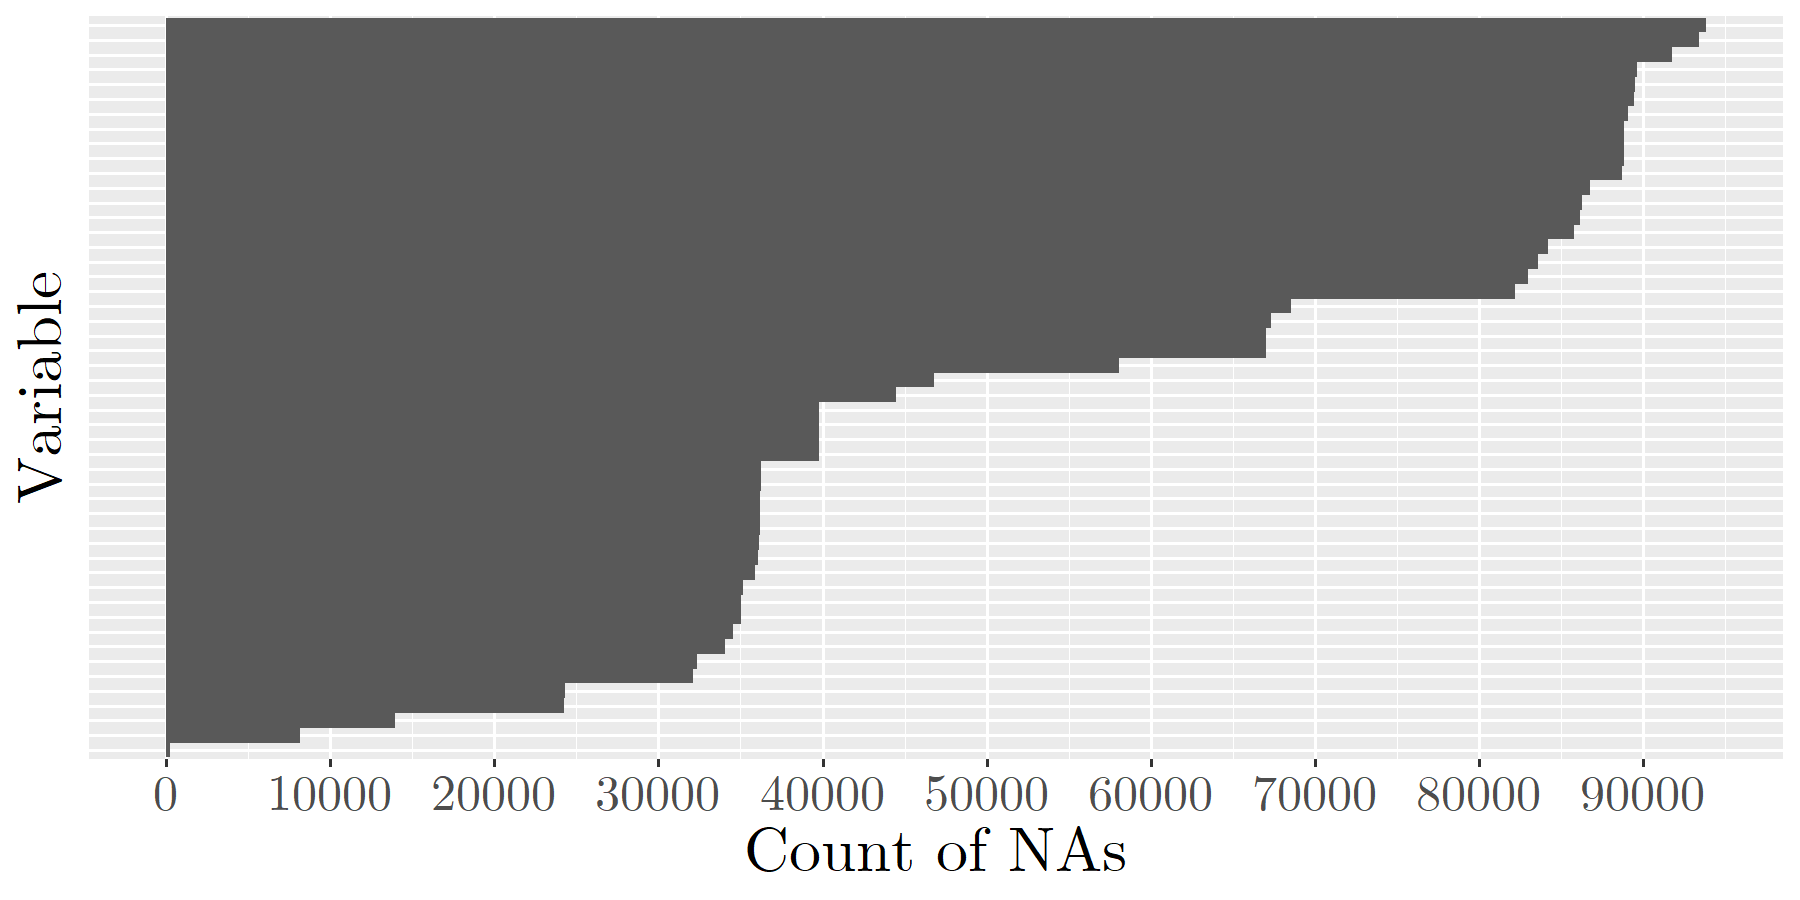
\includegraphics[width = \textwidth]{NABarplot}
	\end{figure}
	
	Given the large number of variables, the variable names have been omitted from the visual. However, some important information can still be gathered. One can see that every variable has at least a handful of missing values. As such, it would be helpful to start with the variables that have the highest count, and see if there are any patterns. There is a steep drop off of the count of NAs at around 75,000 (emphasized with red line), so analyzing all the variables with more than 75,000 NA could give some useful information.
	
	\begin{figure}[H]
		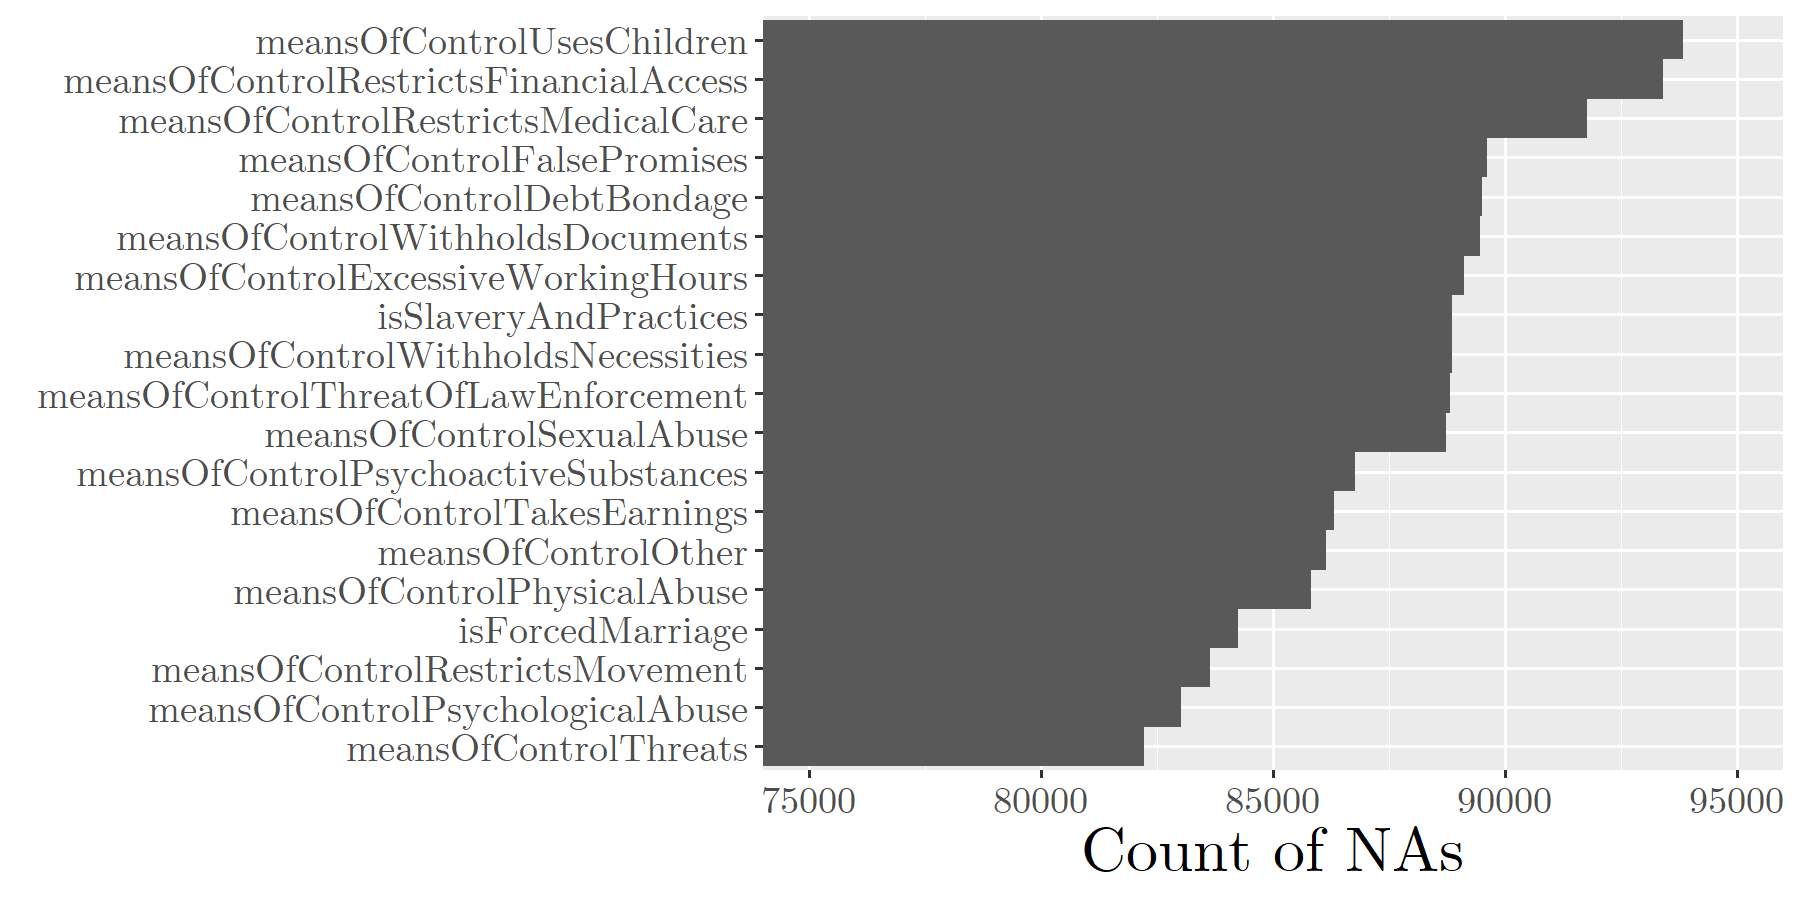
\includegraphics[width = \textwidth]{NABarplot2}
	\end{figure}
	
	From the figure, one can see that the "meansOfControl-" variables take up a large number of spaces on the list. Of the 19 variables with over 75,000 NA values, 17 of them are "meansOfControl-." This could be a direct effect of the way in which the data is recorded. If an individual is transcribing cases to the data set, they may have decided that after determining that one type of control was used, to leave all the other types as "missing." The data set does have a variable that is 1 if there is no specified means of control. We can analyze this variable to determine if it would be worthwhile to modify the data set to salvage the means of control information that does exist.
	
	The "means of control not specified" variable takes a value of 1 if there is no specified means of control. This variable has roughly 50,000 values of 1, and roughly 30,000 values of 0. Meaning that only 30,000 entries in our data set have a means of control specified. By replacing each NA in these variables with 0, we are able to add up all the values for each entry in the data set. This will tell us how many means of control variables are specified.
	
	\begin{figure}[H]
		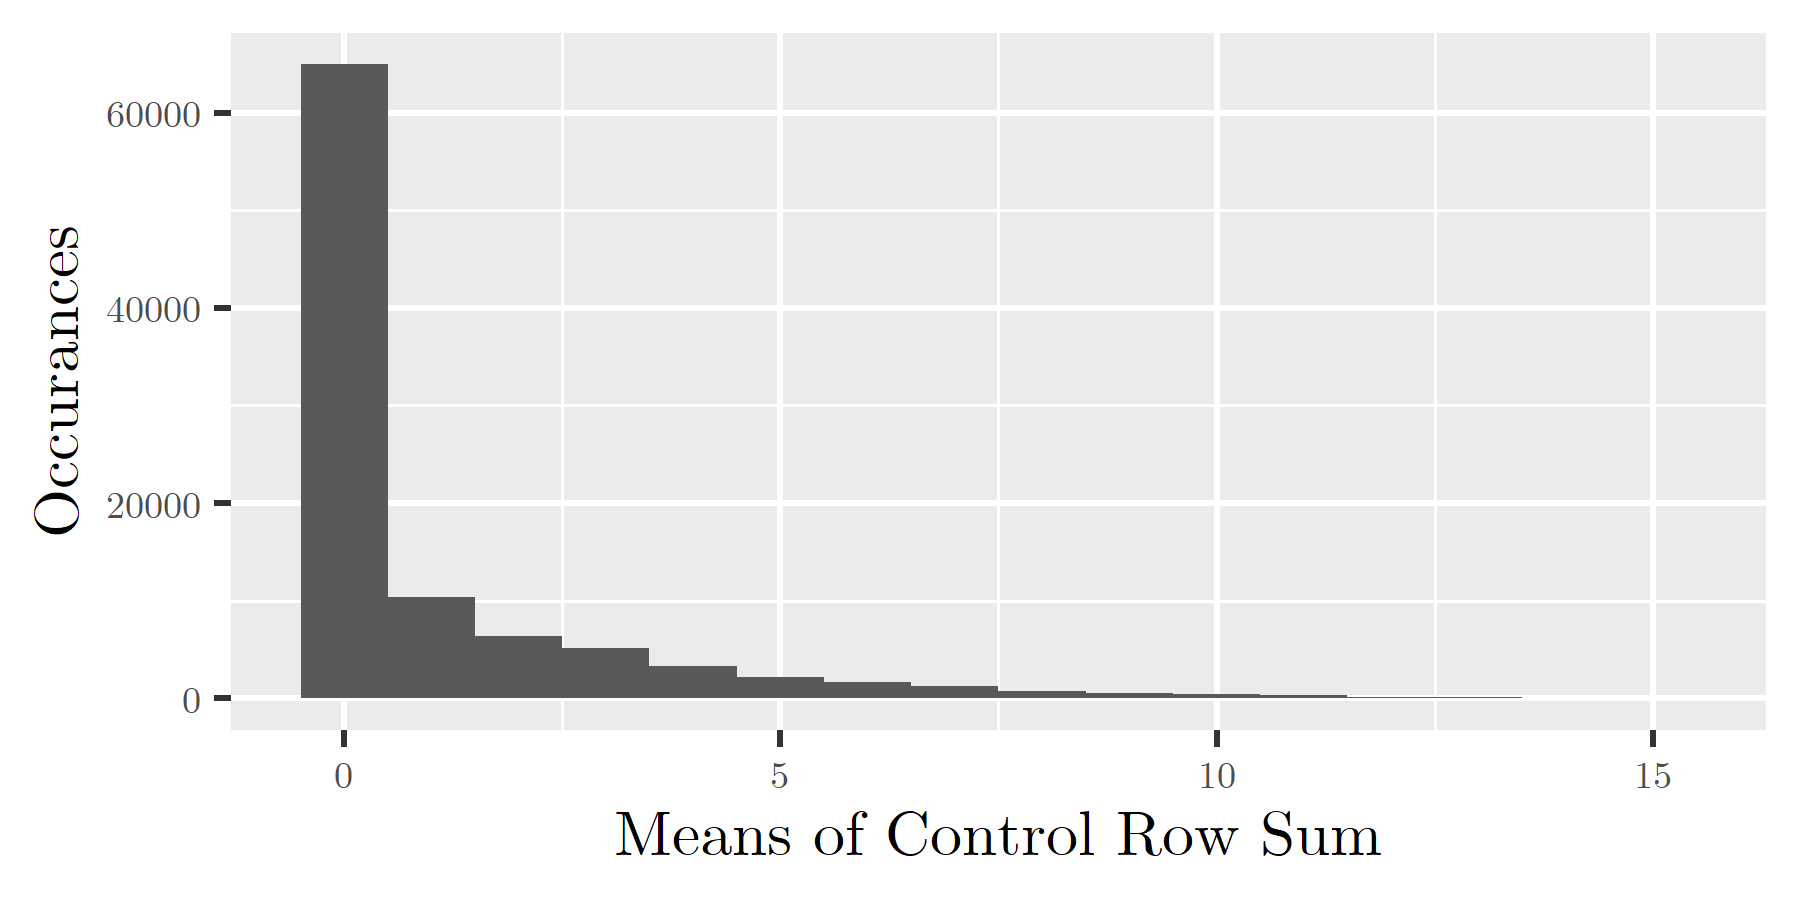
\includegraphics[width = \textwidth]{MeansOfControlSumHist}
	\end{figure}
	
	This histogram allows a visualization of how many instances there are of means of control not being specified. From this histogram, one can see that row sums of 0 are the most common and make up over two-thirds of the data entries. This means that a large proportion of our data cannot even be salvaged by replacing NAs with values of 0. Even if one were to choose to replace the NAs with 0, the sheer lack of recorded entries implies that this data is hard for law enforcement to notice. As such, even if these variables were considered to have a significant effect on model outcomes, there are so many of them that the model would place a higher importance on these types of variables. This is a result of over fitting, and since we want the final model to be applicable and easy to understand, removing these would lead to that goal the quickest.
	
	After removing the Means of Control variables, we are left with 32 variables, and 806 complete entries. This is great progress, but more can be made. To get a better idea of where missing values are, the following visualization is helpful:
	
	\FloatBarrier
	\begin{figure}[H]
		\hspace*{-2cm}
		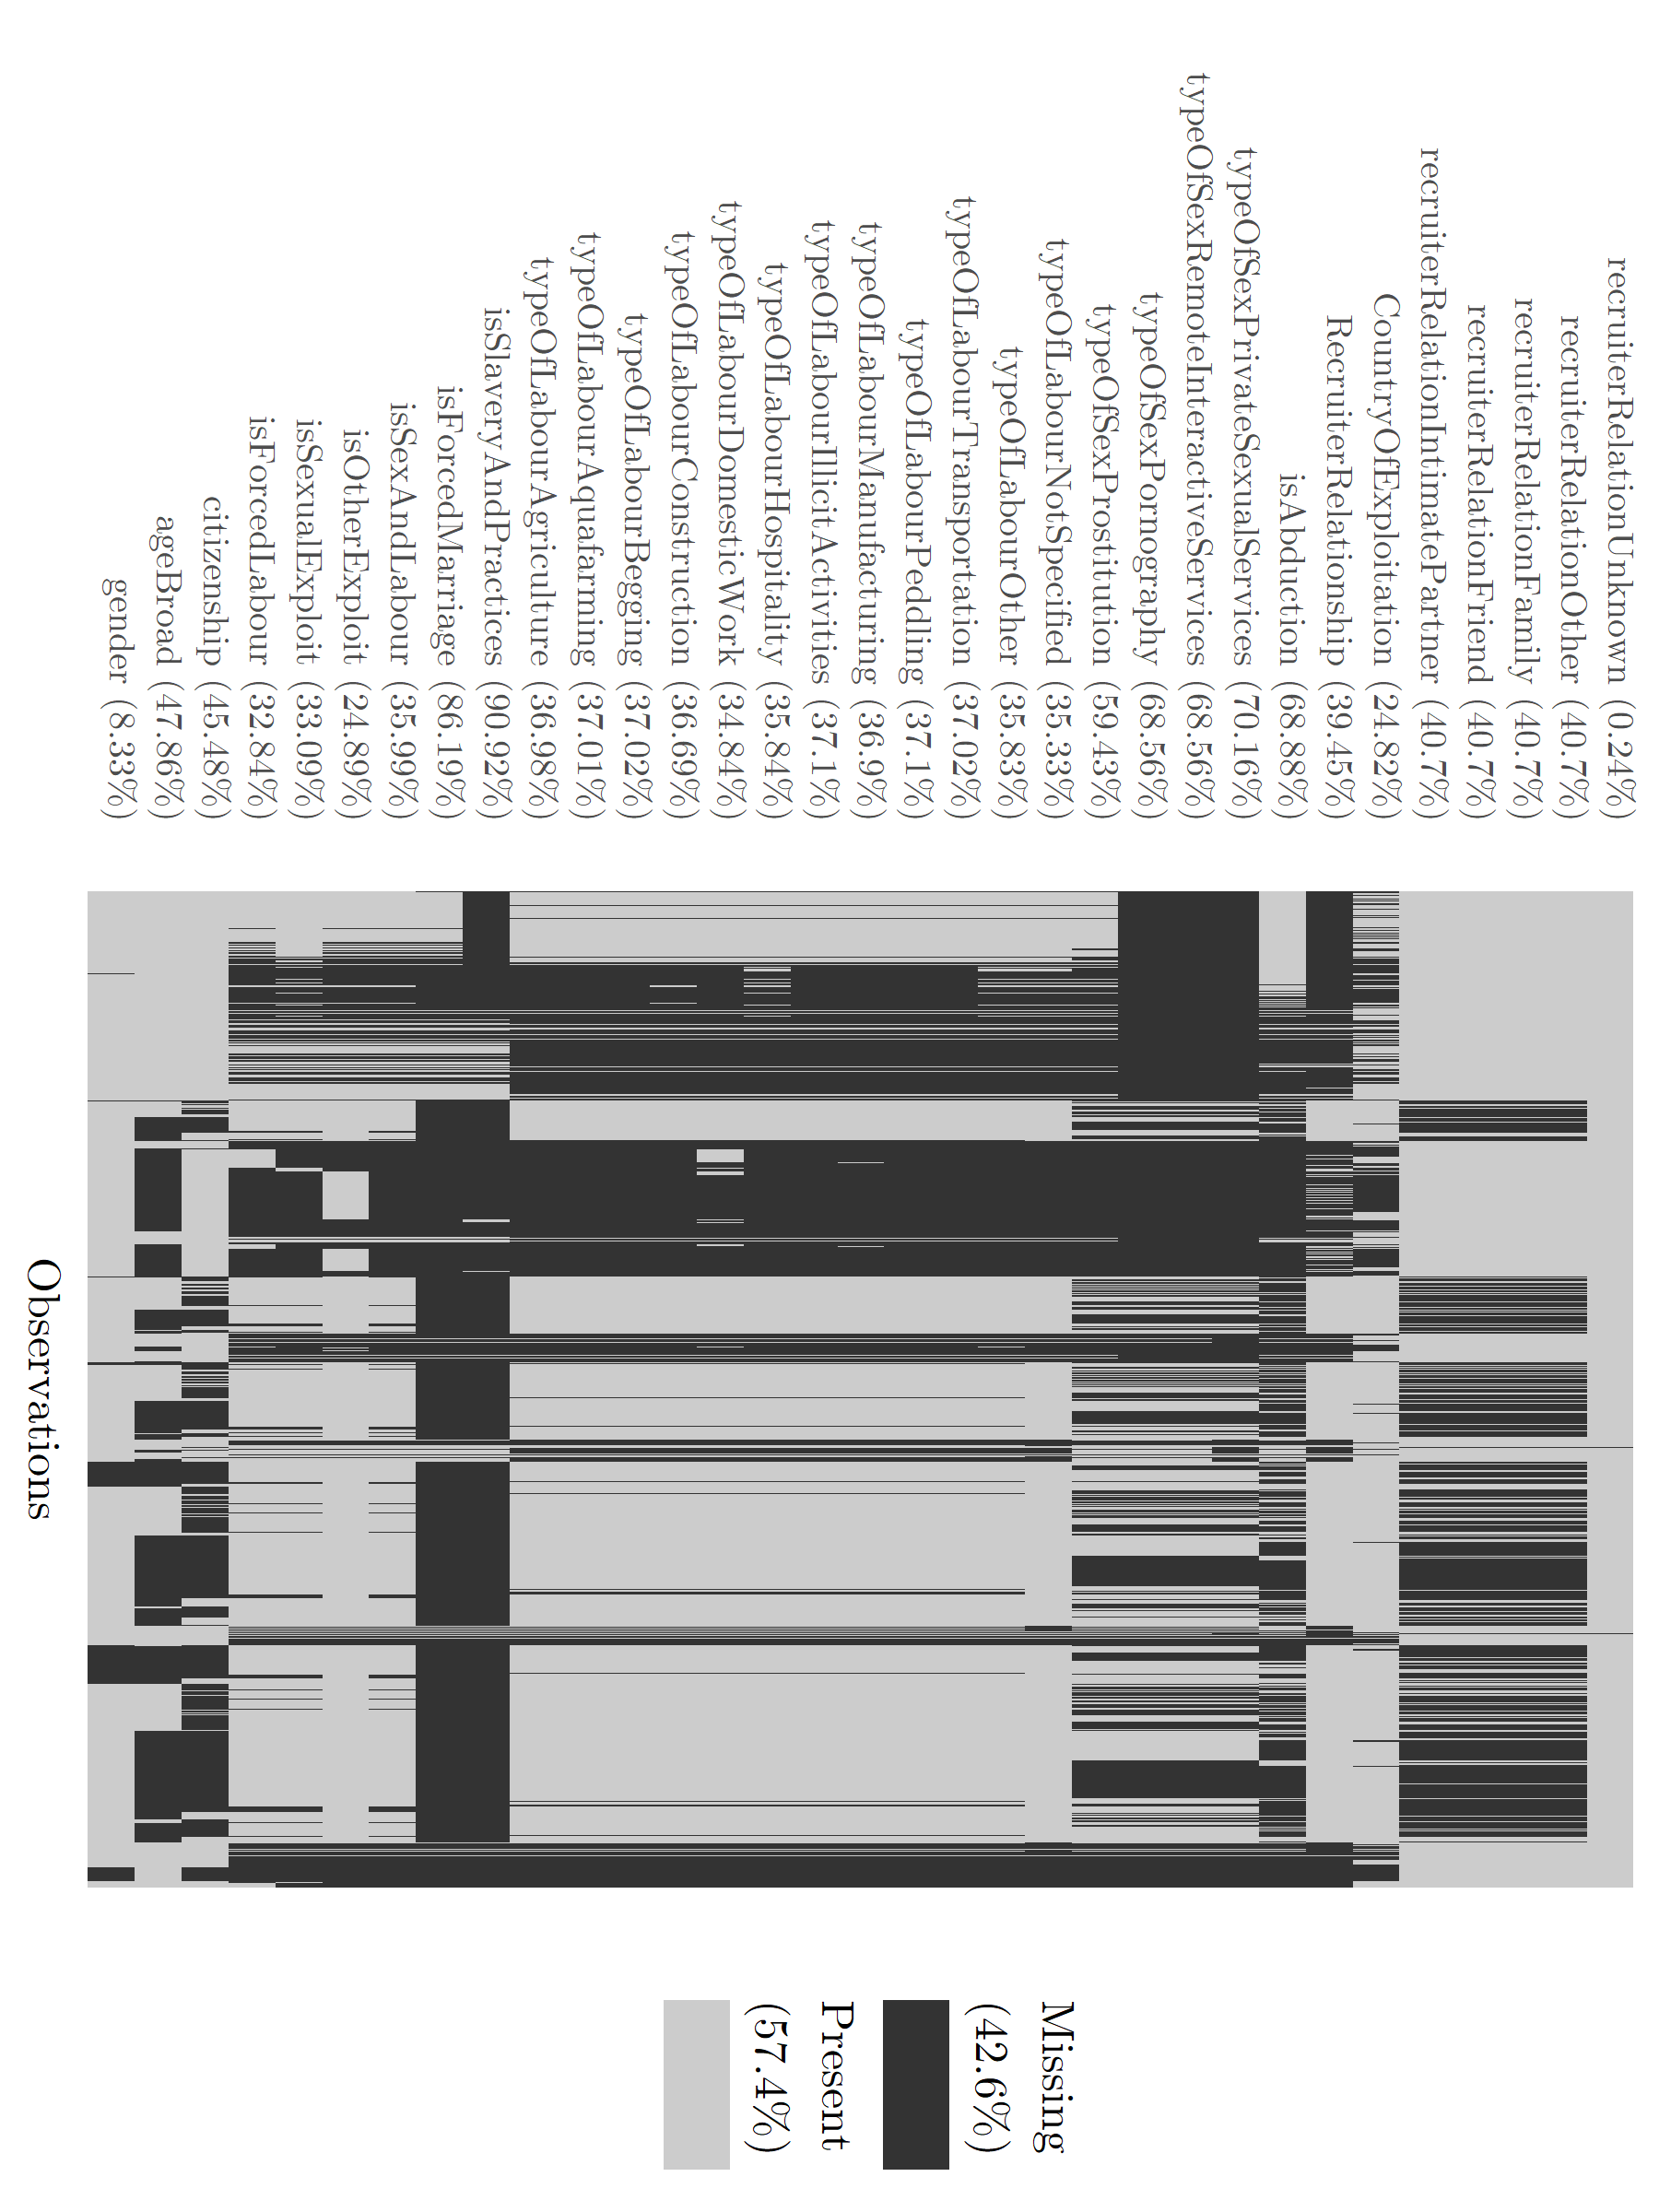
\includegraphics[height = 1.4\textwidth, angle = 90]{NaniarVis1}
		\caption[]{This is a visual of every missing value in the data set. Each row represents a variable and each column represents a case of trafficking. Each black rectangle shows where a missing value is located within the data set}
		\label{fig:Naniar}
	\end{figure}
	\FloatBarrier
In this visual, the missing values for each variable are shown visually. We can see large bands of missing data in both the horizontal and vertical directions. Horizontal bands of missing data correspond to that variable having a lot of missing values. For example, isSlaveryAndPractices is missing 90.92\% of its values, and as such that row seems to be almost entirely black. 

Additionally, there are instances when there seems to be a large correlation between values missing in different variables. An example of this would be the "recruiter relation" variables. In virtually all cases in which one of these variables is missing, all the others are missing as well. This is interesting, as it would imply that if the recruiter relation was known, values of 0 were entered for the recruiter relationships that were not present. This is contrast to the means of control variables, in which NA was evtered even if another means of control was observed. This leads one to believe that there is inconsistent data entry practices within the IOM.

From this visual, we would consider removing "isSlaveryAndPractices", and "isForcedMarriage", as they have percentages of missing values, 90\% and 86\% respectively, that are significantly higher than the other variables. Removing these variables brings the number of complete entries from 806 to 1,424 complete cases. Removing these two variables has more than doubled our number of complete entries.

While 1,424 is enough complete entries to create some meaningful models, it is still only representative of less than 2\% of all the entries in the data set. It would be a good idea to look at some interactions between missing variables, to see if there are any that are missing together as opposed to individually to yield better model results. This can be done with an Upset Plot, as is outlined in \cite{UpsetPlot}.

\begin{figure}[H]
	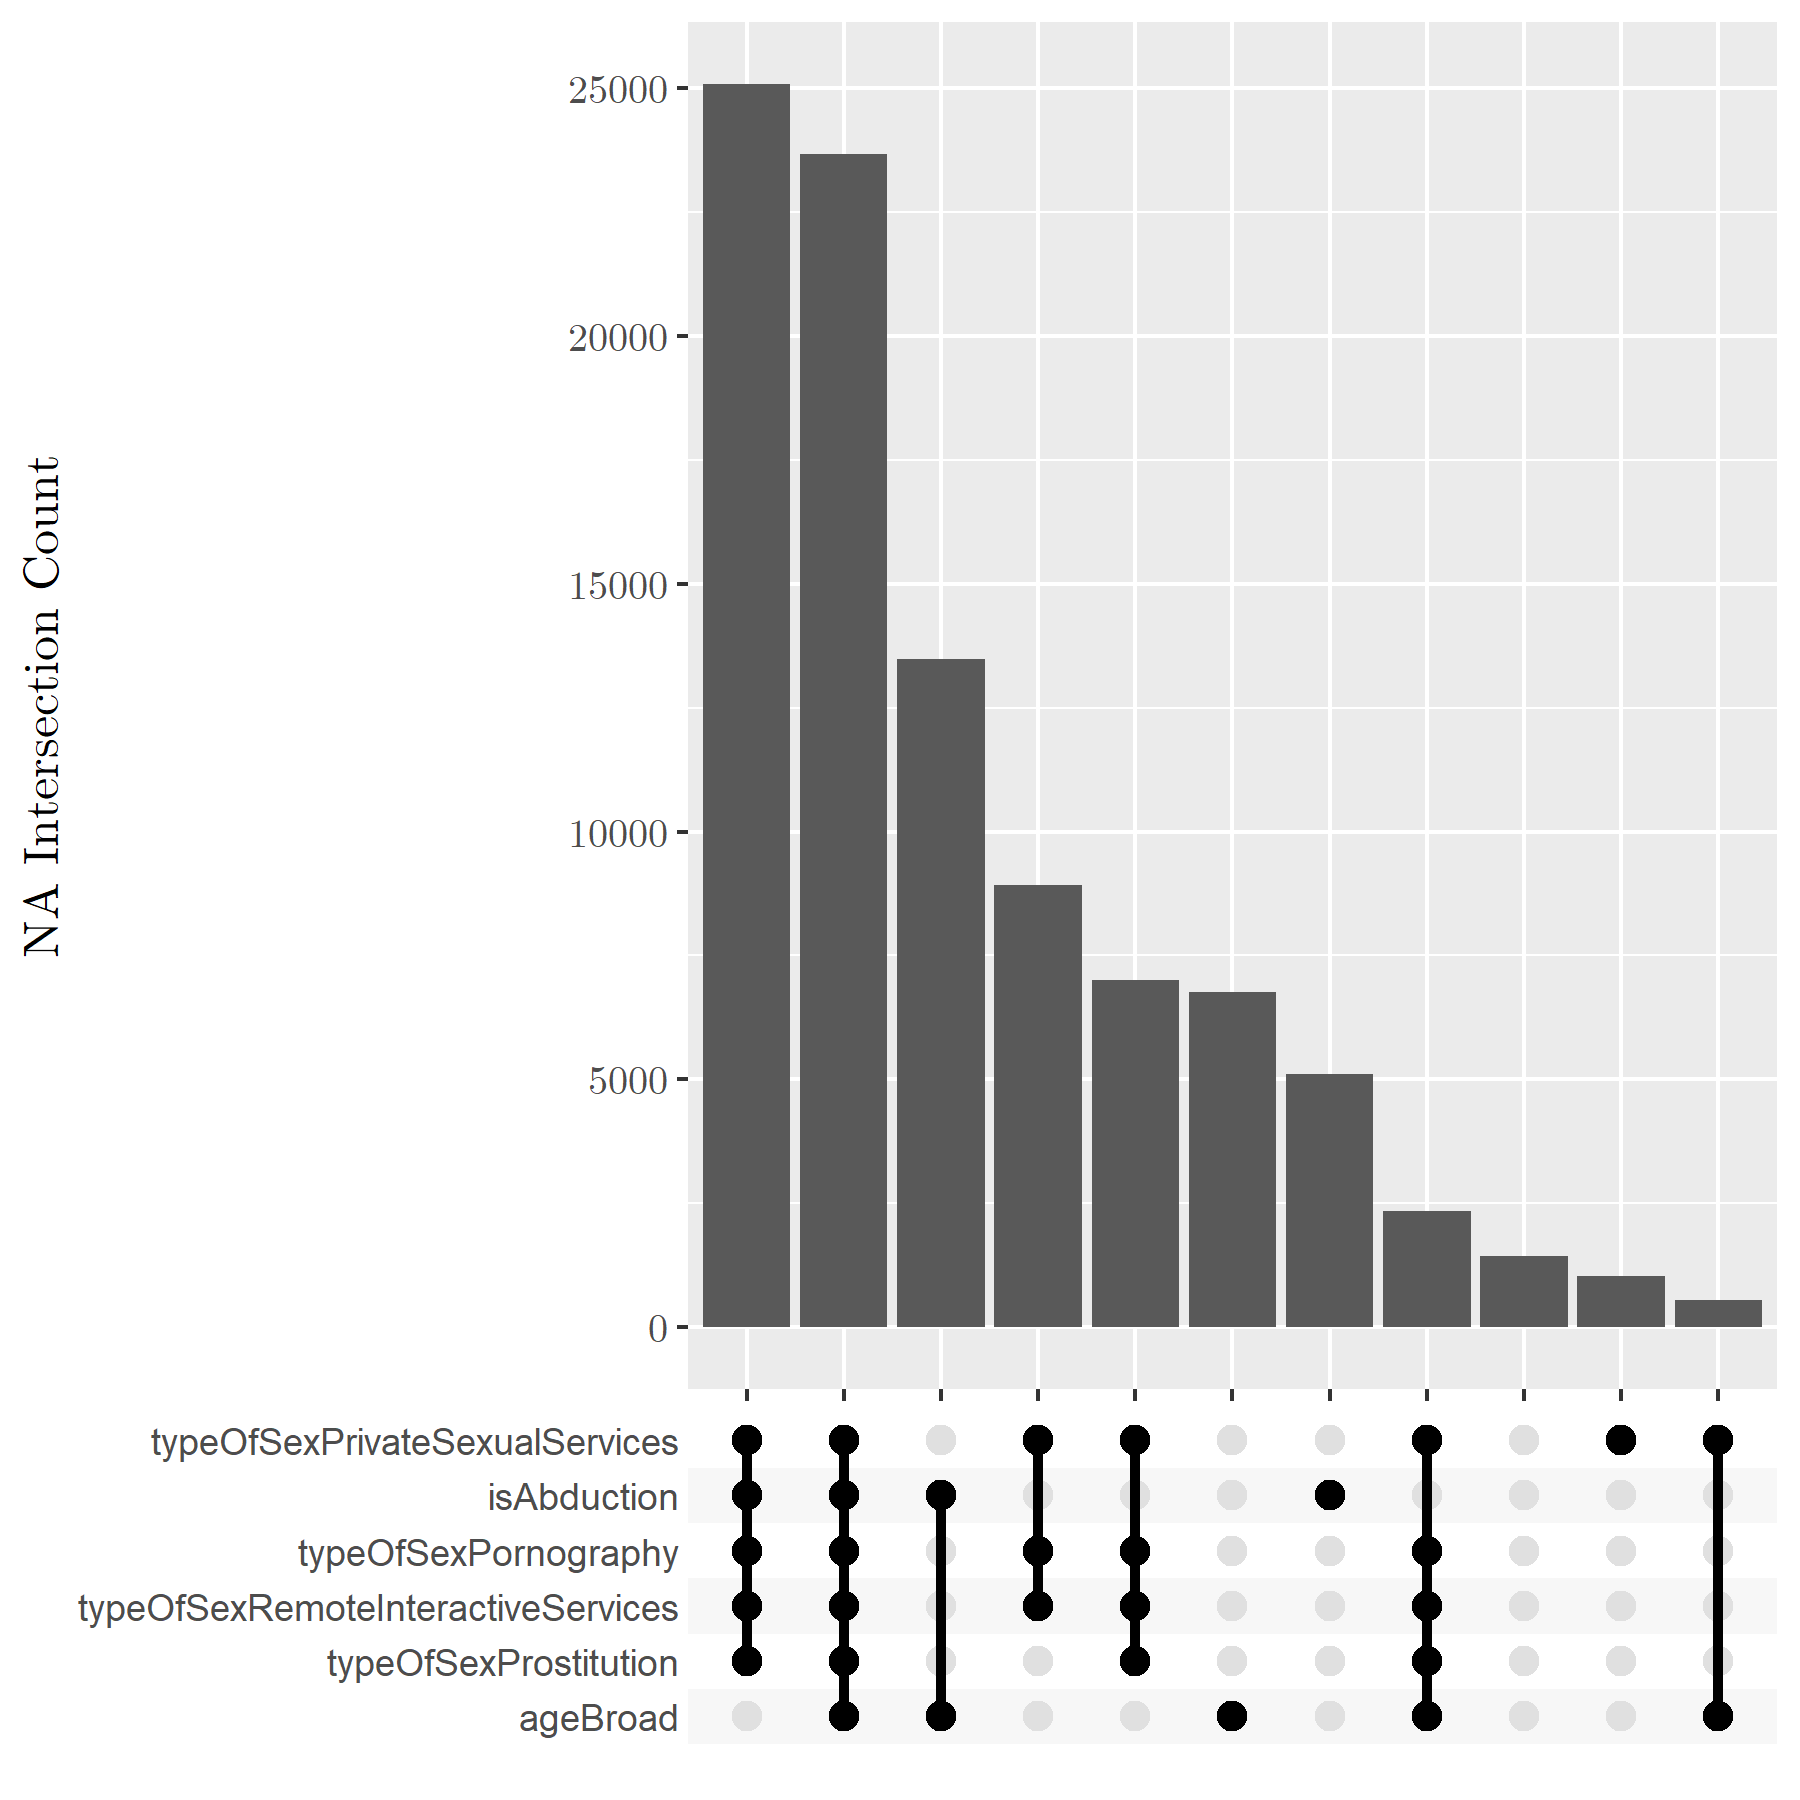
\includegraphics[width = \textwidth]{UpsetPlt1}
	\caption{Count of cases in which every variable selected under the chart is missing}
\end{figure}

From this visualization, along the bottom, one can see which sets of variables lead to the most missing values. For example, the "type of sex" variables and "isAbduction" have a count of roughly 25,000. This means that there are 25,000 rows in our data set that are missing all of those values. This gives us a visual way to determine which variables contribute to incomplete entries, and give us the exact number of rows that are incomplete due to those combinations of variables. Thus, we can attempt to find groups of variables that have a high number of missing rows, but that we also feel would be ineffective metrics that alw enforcement and policy makers can use. 

The first set of variables have over 25,000 incomplete rows; however, removing 4 variables seems like it would be too much, especially since tis group includes "isProstitution" and "isAbduction," both of which are variables that have been shown to be correlated with high rates of human trafficking \parencite{SlaveBook, polarisTypology}. The first set that does not contain either of these two variables is set 4, which contains private sexual services, pornography, and remote interactive services. These are variables that one can feel comfortable removing, as they contribute to a large number of incomplete rows, and are hard to find and prevent from a law enforcement and policy perspective.

Removing these variables yields 6,672 complete cases with 27 total variables. While this process did not take into account the root causes for missing data, later discussion will attempt to determine these causes, and explain what effect it has on the final model. At this point, there are a large enough number of complete entries with a small count of variables, enough for the modeling process to begin.

\subsubsection{Final Removal}

After all the changes made, there are now more colomns in which every value is the same. Naturally, these columns will be removed from the data set, but the number of complete entries will remain he same. These variables are:

\begin{itemize}
	\item Type Of Labour Illicit Activities
	\item Type Of Labour Peddling	
	\item Type Of Labour Transportation
	\item Type Of Labour Not Specified
	\item Is Abduction		
\end{itemize}

The previous methods of data augmentation have allowed us to have a complete data set; however, some unintended consequences of these steps have ultimately occurred. These consequences are not the result of any individual step, but are due to a combination of factors. The most significant contributing factor is perhaps the non-uniform distribution of missing values. This fact is best illustrated when the stages of demographic transision are added to the data set. 

\subsubsection{Augmenting Demographic Transition Data}

As previously mentioned, a country's stage in demographic transition can be determined by looking at a current population pyramid for that country. To accomplish this, the United States Census Bureau has publicly available data of every country \parencite{USCB}, including current population pyramids. By observing these, one can determine a country's current stage in demographic transition. This information was then appended to the CTDC Data Set and will serve as the dependent variable in this research. These values will replace country names in the "citizenship" and "CountryOfExploitation" variables.

\subsubsection{Correlation}

Another metric that will help determine the suitability of the data set is by observing the correlation matrix of all variables. In this matrix, darker squares indicate a stronger correlation between two variables. Places in which the squares are lightest indicate little or no correlation. Additionally, after a hypothesis test is completed, an $\times$ is placed over any combination of two variables with an insignificant correlation (significance level of $p <= 0.05$). This means that any two variables without an $\times$ have a correlation that we can assume to be significantly different from 0.

\FloatBarrier
\begin{figure}[H]
	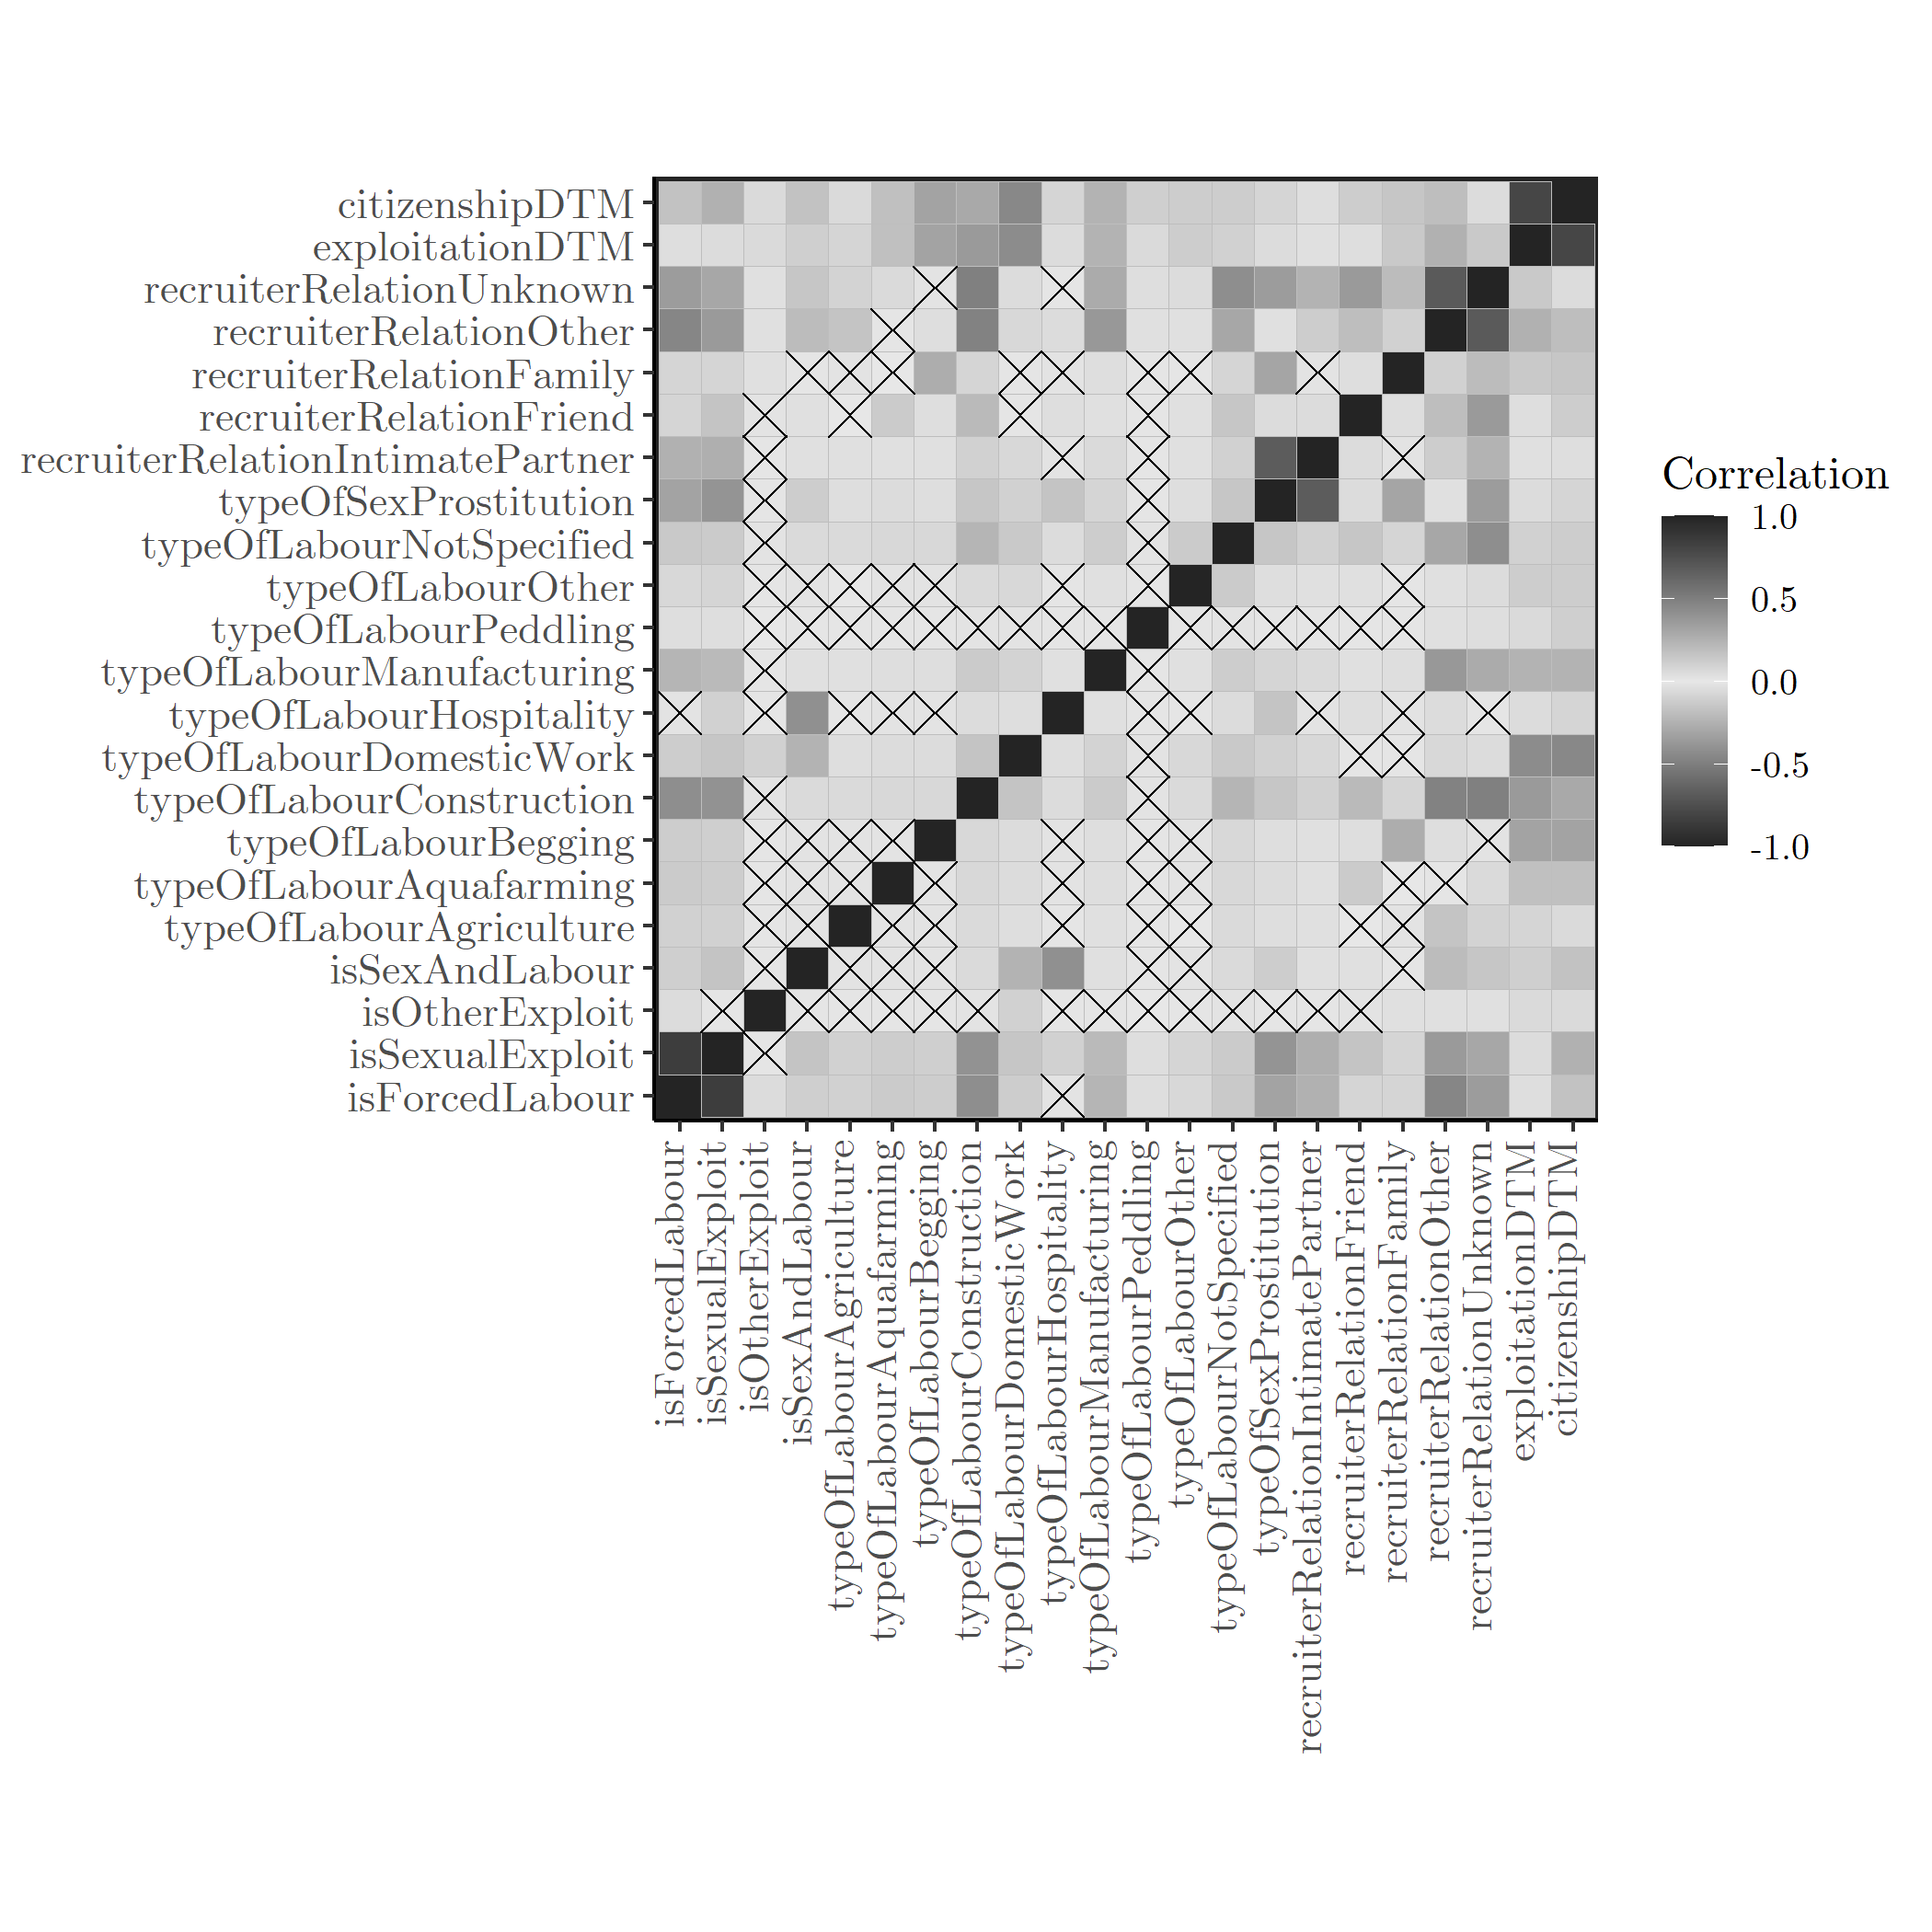
\includegraphics[width = \textwidth]{CorrPlot}
\end{figure}
\FloatBarrier

From the figure, there are no instances of a variable having insignificant correlation with all the other variables. Additionally, there are no observed variables which have a high correlation with all other variables. This is a good sign, because it means there will not likely be any problems of collinearity. Another interesting observation is the fact that citizenshipDTM and exploitationDTM appear to have comparable correlations with each variable in the data set. However, this is to be expected, as we have already shown that cases tend to have the same value for both variables. 

Already from this plot, we can see that the exploitatioDTM of a country is most correlated with typeOfLabourDomesticWork and typeOfLabourConstruction. The same is true for citizenshipDTM, and since there are no variables that are insignificantly correlated with all other variables, there is no need to make any major augmentations to the data set. This means that the data set could be a contender for creating thorough and significant models.

\subsubsection{Individual Country Over-representation}

Since the data set has only 4 categories for DTM stage, we need to ensure that none of the stages are being over represented by one specific country. If all of our stage 2 entries originate from one country, then we cannot logically conclude the model will generalize for all countries, and this is where a major problem of the previous steps emerges.

\FloatBarrier
\begin{figure}[H]
	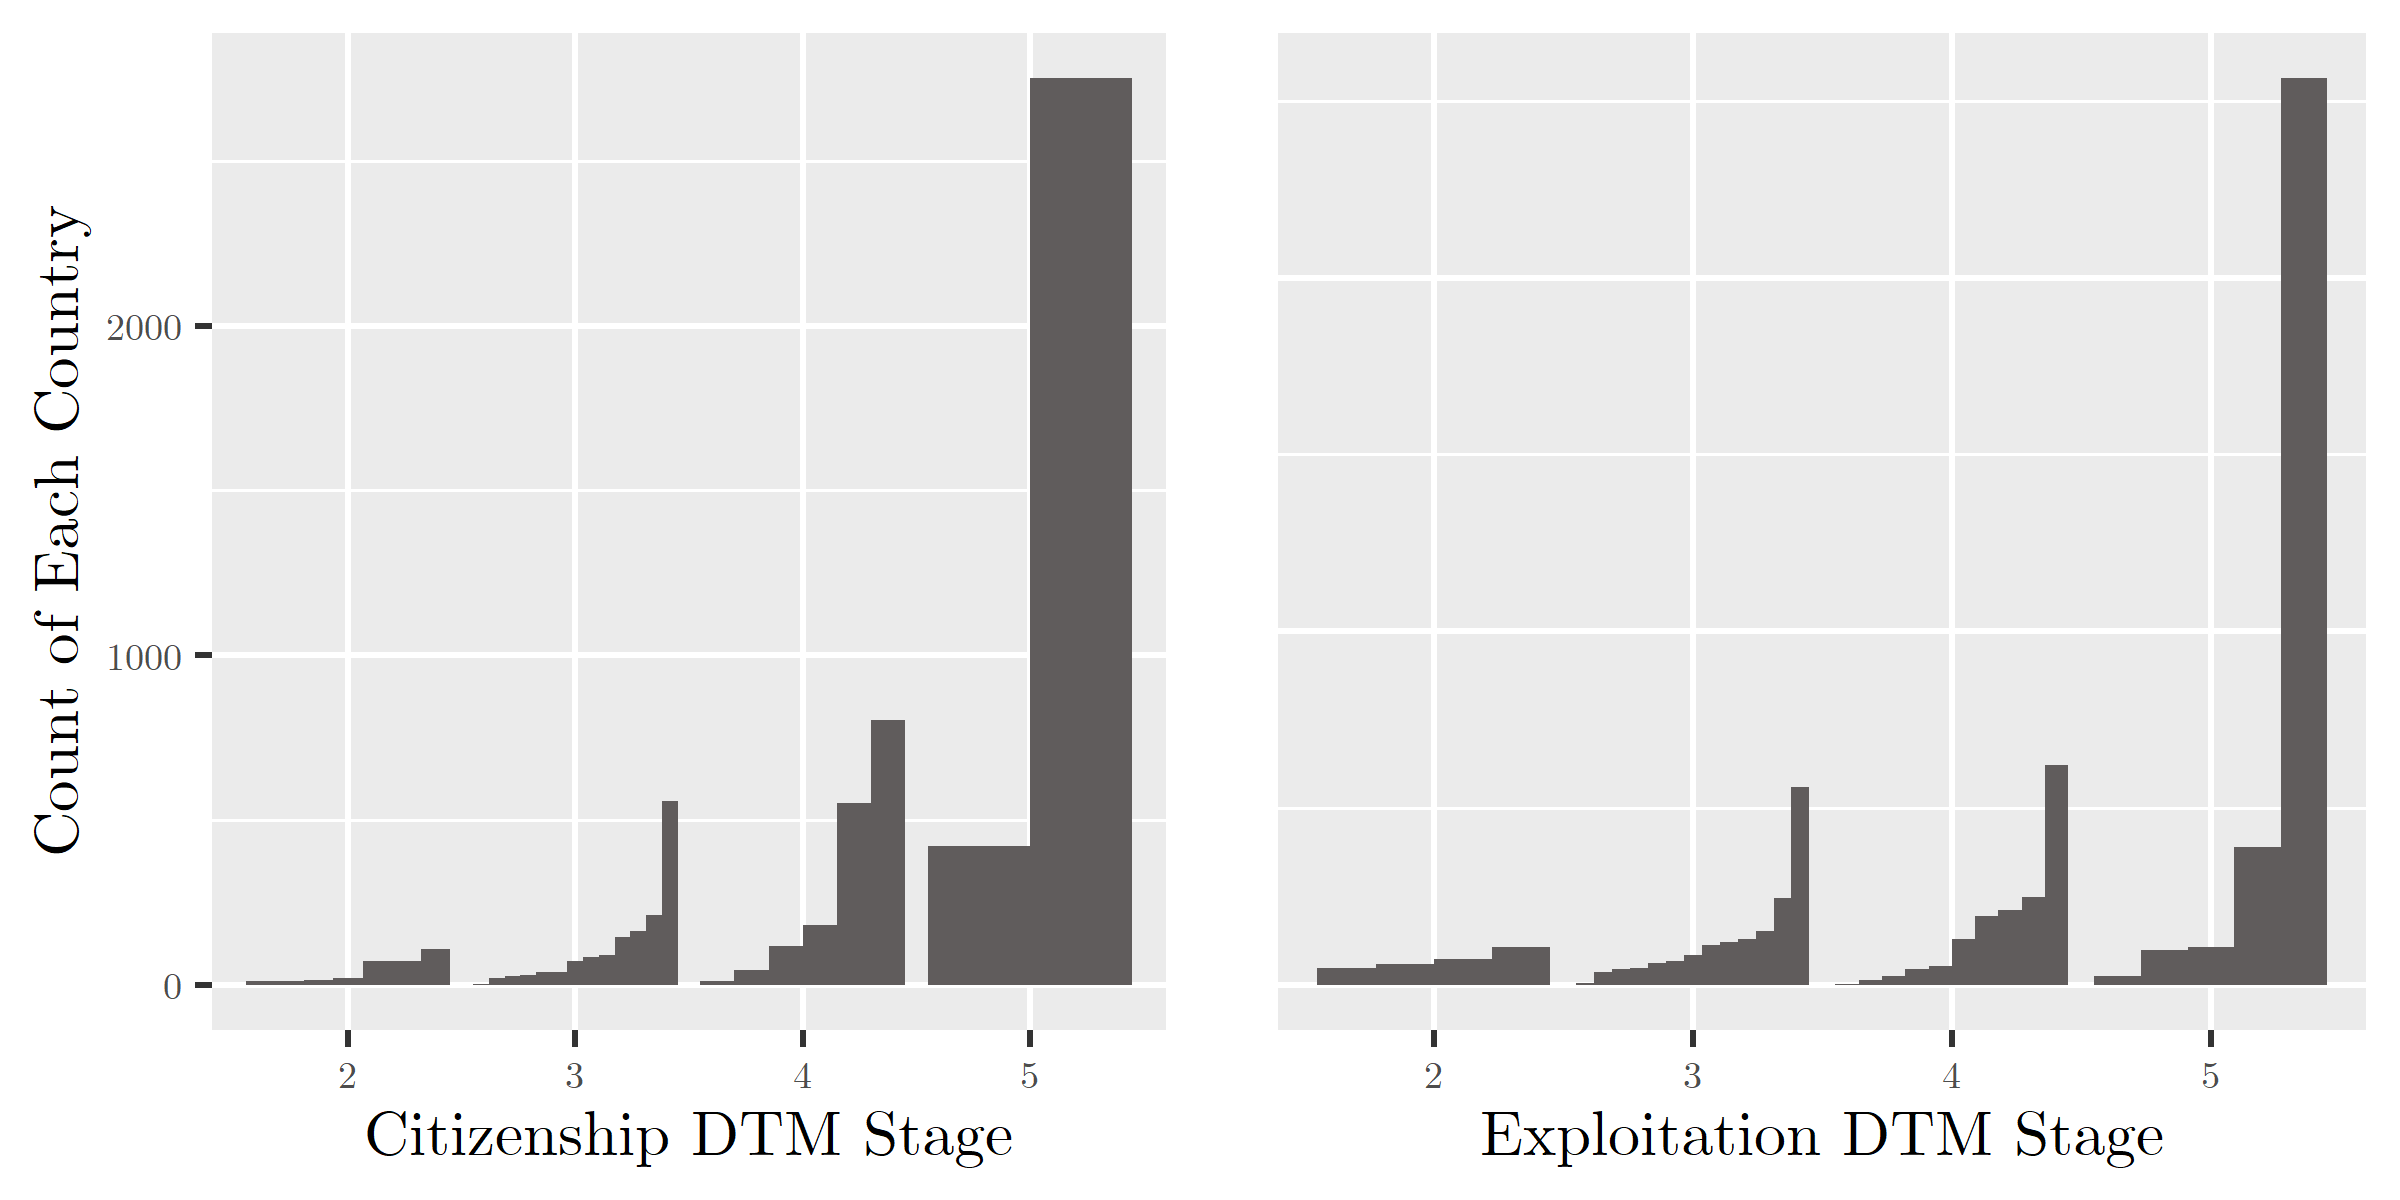
\includegraphics[width = \textwidth]{CountryCountBarplot}
\end{figure}
\FloatBarrier

In these bar plots, each bar corresponds to an individual country, and the height of the bar shows the count of that country in the data set. In both cases, there seems to be no countries that overpower stages 2, 3, \& 4. However, in both graphs, there seems to be one country in stage 5 that has significantly more entries than the other stage 5 countries. In order to determine if this will effect any modeling, one would need to analyze the data of the countrys in question, and determine if there is enough variation in the data to still use it. 

From further analysis, it is determined that the stage 5 citizenship country with a high count is UA (Ukraine), and the high count in the stage 5 exploitation countries corresponds to RU (Russia). Since these two countries have a history of conflict, future research may yield interesting findings, given that the data set has so many entries. Additional modeling could be completed purely on Ukranian citizens who are exploited in Russia. However, this has been a long known phenomenon, in which Ukrainian citizens are exploited in Russia. This data set predates the 2022 war between Ukraine and Russia, but it has been noted that the Russian government likely has some involvement in the trafficking of persons, hence why it is so widespread in the country \parencite{RussiaTrafficking}.

While further analysis of Ukraine and Russia would be interesting, the overall goal is to create a general model for all countries. To determine if the effect of these two countries is too strong, we need to determine if there is a significant difference between the overall data structure between these countries, and other stage 5 countries. This can be achieved with a Chi-Square test.

For the sake of the Chi-Square test, we will have two groups of entries in the data set. Group A will be all entries which are the over represented country, and group B will be all other countries that are in the same stage. A Chi-Square test can look at each variable, and determine if there is a significant difference between the two groups for that variable. Since one group is exclusively made up of one country, this will show if that one country has a significant difference between other countries of the same stage. From this, we would ideally see that there is no significant difference between the groups in regards to any variable. 

However, the Multiple Comparisons Fallacy is likely to be present. This means that for any large group of data, if a significance test is completed over every variable, eventually a significant P-Value will be found (or insignificant depending on the case). What this means for the following test is that we are hoping to find many instances of there being no significant difference between the groups, but there may be one or two insignificant p-values, and this does not discredit the entire analysis. This is further explained in \cite{Fallacy}.

For the following Chi-Square tests, the null hypothesis is that group A and B not significantly different, and the alternative is that they have do have significant differences for that variable. That means that a significant p-value means that there is a significant difference between the groups. Additionally, not every variable will appear in the table, those that are omitted have the same value for all entries, and thus a test would not be possible, and would not give any meaningful information.
\FloatBarrier
\begin{table}[!ht]
	\centering
	\caption{$\chi^2$ Comparing Russia to Other Stage 5 Countries of Exploitation}
	\begin{tabular}{lccc}
		\toprule
		\bf{Variable Name}        & \boldmath{$\chi^2$} \bf{Statistic} &  \boldmath{$p$}   & \boldmath{$p<0.05$} \\ \midrule
		gender                    &               609.9                & \num{1.177e-134}  &   \boldmath{$*$}    \\
		ageBroad                  &               482.9                & \num{3.804e-100}  &   \boldmath{$*$}    \\
		isForcedLabour            &               621.4                & \num{3.801e-137}  &   \boldmath{$*$}    \\
		isSexualExploit           &               621.4                & \num{3.8014e-137} &   \boldmath{$*$}    \\
		typeOfLabourAgriculture   &                14.5                &  \num{1.405e-04}  &   \boldmath{$*$}    \\
		typeOfLabourConstruction  &               297.1                &  \num{1.443e-66}  &   \boldmath{$*$}    \\
		typeOfLabourDomesticWork  &                61.5                &  \num{4.507e-15}  &   \boldmath{$*$}    \\
		typeOfLabourHospitality   &                57.3                &  \num{3.750e-14}  &   \boldmath{$*$}    \\
		typeOfLabourManufacturing &                2.9                 &    \num{0.085}    &                     \\
		typeOfLabourOther         &                4.3                 &    \num{0.037}    &   \boldmath{$*$}    \\
		typeOfLabourNotSpecified  &                35.5                &  \num{2.595e-09}  &   \boldmath{$*$}    \\
		recruiterRelationFriend   &                68.5                &  \num{1.280e-16}  &   \boldmath{$*$}    \\
		recruiterRelationFamily   &                0.1                 &    \num{0.724}    &                     \\
		recruiterRelationOther    &               131.4                &  \num{2.050e-30}  &   \boldmath{$*$}    \\
		recruiterRelationUnknown  &               265.4                &  \num{1.147e-59}  &   \boldmath{$*$}    \\ \bottomrule
	\end{tabular}
\end{table}

\begin{table}[!ht]
	\centering
	\caption{$\chi^2$ Comparing Ukraine to Other Stage 5 Countries of Citizenship}
	\begin{tabular}{lccc}
		\toprule
		\bf{Variable Name}        & \boldmath{$\chi^2$} \bf{Statistic} &  \boldmath{$p$}  & \boldmath{$p<0.05$} \\ \midrule
		gender                    &               390.4                & \num{1.674e-85}  &   \boldmath{$*$}    \\
		ageBroad                  &               950.4                & \num{6.812e-194} &   \boldmath{$*$}    \\
		isForcedLabour            &               695.4                & \num{9.878e-152} &   \boldmath{$*$}    \\
		isSexualExploit           &               695.4                & \num{9.878e-152} &   \boldmath{$*$}    \\
		typeOfLabourAgriculture   &                11.6                & \num{2.961e-03}  &   \boldmath{$*$}    \\
		typeOfLabourConstruction  &               229.2                & \num{1.725e-50}  &   \boldmath{$*$}    \\
		typeOfLabourDomesticWork  &                50.7                & \num{9.973e-12}  &   \boldmath{$*$}    \\
		typeOfLabourHospitality   &                35.1                & \num{2.4445e-08} &   \boldmath{$*$}    \\
		typeOfLabourManufacturing &                81.9                & \num{1.652e-18}  &   \boldmath{$*$}    \\
		typeOfLabourOther         &                4.2                 &   \num{0.121}    &                     \\
		typeOfLabourNotSpecified  &                29.3                & \num{4.416e-07}  &   \boldmath{$*$}    \\
		recruiterRelationFriend   &                30.6                & \num{2.267e-07}  &   \boldmath{$*$}    \\
		recruiterRelationFamily   &                1.4                 &   \num{0.487}    &                     \\
		recruiterRelationOthe     &               340.9                & \num{9.269e-75}  &   \boldmath{$*$}    \\
		recruiterRelationUnknown  &               435.1                & \num{3.345e-95}  &   \boldmath{$*$}    \\ \bottomrule
	\end{tabular}
\end{table}
\FloatBarrier
From the test for stage 5 exploitation countries (Table 1), one can see that there is a significant difference between the two groups for 13 out of the 15 variables being tested. This means that there is a significant difference between Russia and other stage 5 exploitation countries. This means we have an over representation problem, in which one subset of stage 5 countries (Russia) is having a significant effect on our overall data set. This is comparable to sampling bias, and similar measures can be used to combat the issue. Also note that these results are only a problem due to the large number of entries. If we had determined that the countries were not significantly different, then no action would need to be taken. It is due to the large number of entries and the lack of similarities that are the root of the issue, neither one of these facts is an issue on its own.

Similarly, in Table 2 we see the same problem arises with Ukraine, despite there being more stage five countries represented in citizenship than with country of exploitation. Since these are both instances of oversampling from one population (Ukrainian citizens and Russian exploits), this can be counteracted by applying a weight to these instances in the data set. Another solution would be to randomly select entries in which Russia is the country of exploitation or Ukraine in the same of citizenship. This allows us to bring the raw sample count down so that these countries are not over represented.

The process of weighting means that instead of letting these countries (Russia and Ukraine) have the same effect on the model as other countries in their respective categories of exploitation and citizenship, one can assign a weight to these cases. This weight would be less than 1, since we want these cases to have a smaller effect on the model. This process is outlined in \cite{Oversample}, and would be implemented in the modeling phase.



\subsubsection{Conclusions From Removing Causes of Missing Data}

Initially, the act of creating complete entries was done so in an effort to reduce computational time, simplify data analysis, and allow simple model creation. However, in doing so, a combination of factors has led to the creation of a biased data set. Looking again at figure \ref{fig:Naniar}, one can see that the distribution of missing values is extremely non-uniform, implying that there may be a significant effect that other variables have on a variable being missing. For example, it could be that every case located in a particular country may have the same value missing. Additionally, there are some cases in which most values are missing. This could be cause for concern, but is not an insurmountable issue.

The second major problem is the over-representation of Russia and Ukraine, this could be due to having a larger number of cases than other stage 5 countries, or it could also be indicative of data reported from these countries containing more information and fewer missing values. Either way, the oversampling of these two countries is extremely significant, and is cause for concern. While it would be possible to solve this problem by selecting a sub-sample of these entries for our data, this would greatly reduce the number of usable entries, and would lead to ineffective and insignificant models. It is for these reasons that the process ofcreating a data set that implements "missing-ness" as a variable, in hopes of creating a larger data set. 

\subsection{Quasi-Variable Representation of Missing Values}

To start, the initial large data set will be revisited. With 63 columns and 0 complete entries, we will now begin the process of creating a second potential data set for modeling. This data set will attempt to implement information gained from knowing which variables are missing, instead of ignoring missing data entirely.

\subsubsection{Salvaging Missing Data}

To start, the summary variables will be removed, for the same reasons as mentioned previously. These variables serve as a text summary of other attributes of a case which are already recorded as binary data. These removed variables are:

\begin{multicols}{2}
	\begin{itemize}
		\item Means of Control Concatenated
		\item Type of Exploit Concatenated
		\item Type of Labour Concatenated
		\item Recruiter Relationship
	\end{itemize}
\end{multicols}

After removing these variables, each missing value (NA) in the data set is assigned a value of -1. This allows us to have a simple way to notate and keep track of which values are missing. A value of -1 is not a possible value anywhere in the data set, so we can safely use it to denote when a value is missing. A good objective would be to replace some of these missing values with values of 0 or 1. To begin this, it was realized that there were many instances of missing variables in a variable category (such as type of labour), even when other values were recorded as 1 in that category. It is believed that this is a result of individuals recording data into the database only putting values of 1, but not values of 0 into the data set. It is impossible to know exactly how the data was recorded, but simple assumptions such as these must be made in order to gather useful information we otherwise would not have.

There are many instances in the data set in which a value of 1 is recorded for a sub-variable within certain variable categories, and all other variables in the category are missing. It is reasonable to assume that this is potentially a mistake, and these missings should actually be zeros. So each row in the data set was checked, and instances such as these were "salvaged" by replacing the missing values with 0. The following table outlines the number of rows that were salvaged in each category of variables.

\FloatBarrier
\begin{table}[!ht]
	\centering
	\caption{Number of Salvaged Rows By Category}
	\begin{tabular}{cc}
		\toprule
		 Variable Category  & Number of Salvaged Rows \\ \midrule
		Sexual Exploit Type &           31            \\
		Labour Exploit Type &          3,979          \\
		 Means of Control   &         80,325          \\
		Recruiter Relation  &         39,561          \\ \bottomrule
	\end{tabular}
\end{table}
\FloatBarrier
We can see from the table that there were many instances in the data set in which one sub category or type was observed, and others were left as missing. this is understandable as it could be a truly unknown value, but since the goal is to inform law enforcement on what they should be looking for, if a value is unknown when the victim is saved, it is logical to conclude it could not have been observed by law enforcement. However, it is still important to gain some more insight into where the missing values occur.

First, we can visualize which rows were salvaged in the table, and seeing if these correspond to particular countries.

\FloatBarrier
\begin{figure}[H]
	\caption{Types of Rows Salvaged By Country}
	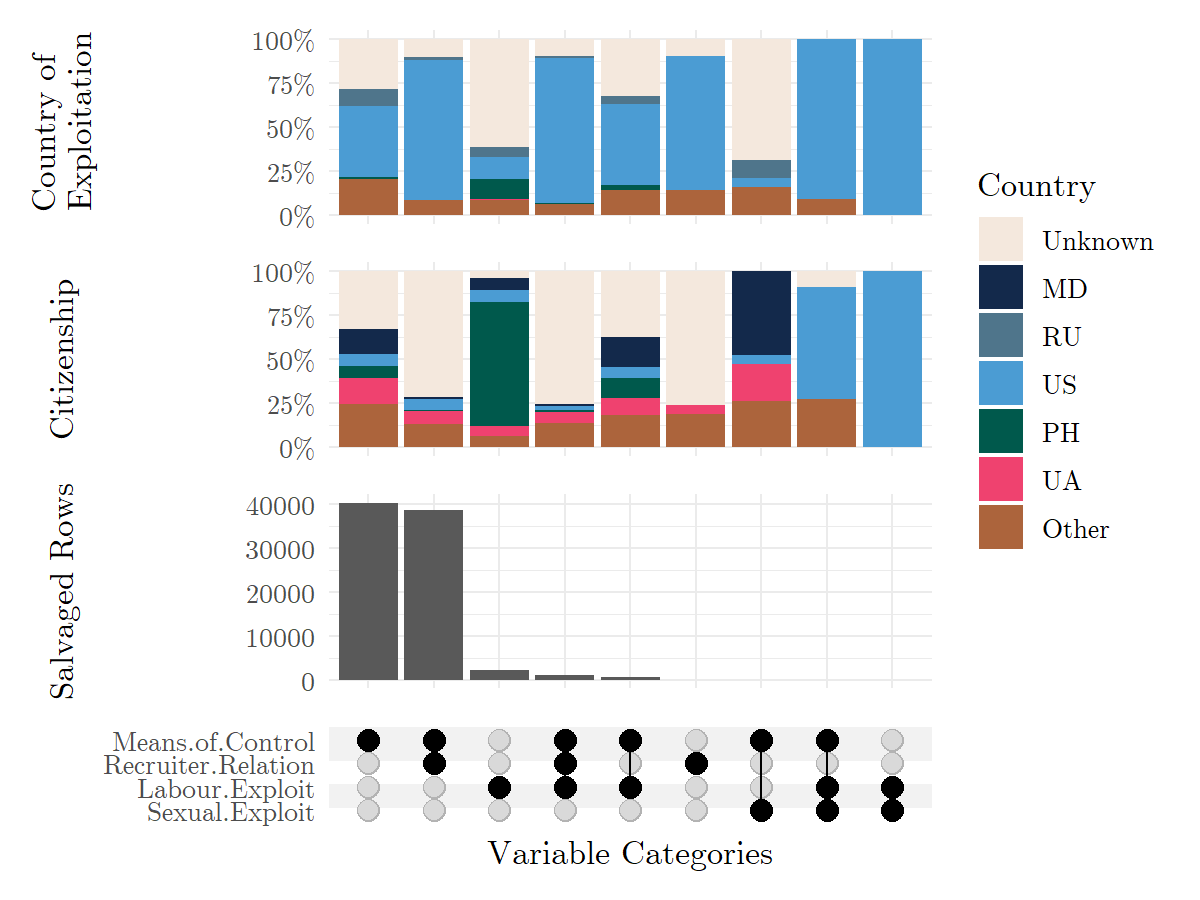
\includegraphics[width = \textwidth]{SalvageRowsUpset}
\end{figure}
\FloatBarrier

To break down this figure, we start with the bottom section that consists of circles. On the left of this section is a variable category such as Labour Exploit and Recruiter Relation. As previously mentioned, all of these categories include binary variables for different aspects of the category. Aspects such as if the labour exploit was in agriculture, and if the recruiter was a family member. In each column of the plot, the dark circles indicate which combination of these categories were salvaged. For example, column 1 corresponds to rows in which Means.Of.Control was the only salvaged category, and column 2 corresponds to rows in which Means of Control and Recruiter relation were both salvaged.

The next section, "Salvaged Rows" simply provides a bar plot that counts the number of rows that were salvaged for each category combination. Finally, the Citizenship and Country of Exploitation sections give a percentage of the salvaged rows that were made up by certain countries. Only the 5 most common countries that make up the salvaged rows are noted, with all other countries being represented by "Other" and NA values as "Unknown".

From the visual, we also see that the most frequently salvaged rows are the ones involving Means of Control and Recruiter relation. This means that these variables were initially underrepresented in the data. This could be due to the fact means of control and recruiter relation are often overlooked in the realm of investigatory knowledge and victim assistance. This is not an unexpected result, as it is often the case in the United States and many other countries, that the manner in which a victim is exploited is perceived as more important than what led to the victim being exploited to begin with. This phenomenon is further explored in \cite{MediaRep}.

Some surprising information gathered from this visual is the fact that the United States (US) is the largest contributing exploitation country to these instances of salvageable row. As a reminder, a row can only be salvaged if a value of 1 is recorded for a sub variable, and there are other variables that have missing values. This implies that the United States records data on victims in such a way that if an aspect of trafficking is not observed, it is not immediately assigned a value of 0. This may appear to be an issue of "sloppy" or inefficient record keeping, but it is also likely that if an aspect of trafficking is not observed, there is no way to truly know if it happened. For example, if a victim is rescued and it was observed that the victim was labor trafficked in an agricultural setting, there is truly no way to rule out if the victim was also trafficked in a construction setting. 

This reasoning seems fairly straightforward and reasonable; it eliminates instances of type II errors (false negatives) as a result of difficulty investigating trafficking. These errors could even occur as a result of a victim's inability to communicate or even remember their experiences, which is a frequent occurrence among victims of trafficking \parencite{PTSD}. 




\subsection{DTM Stages Data}

\FloatBarrier
\begin{figure}[H]
	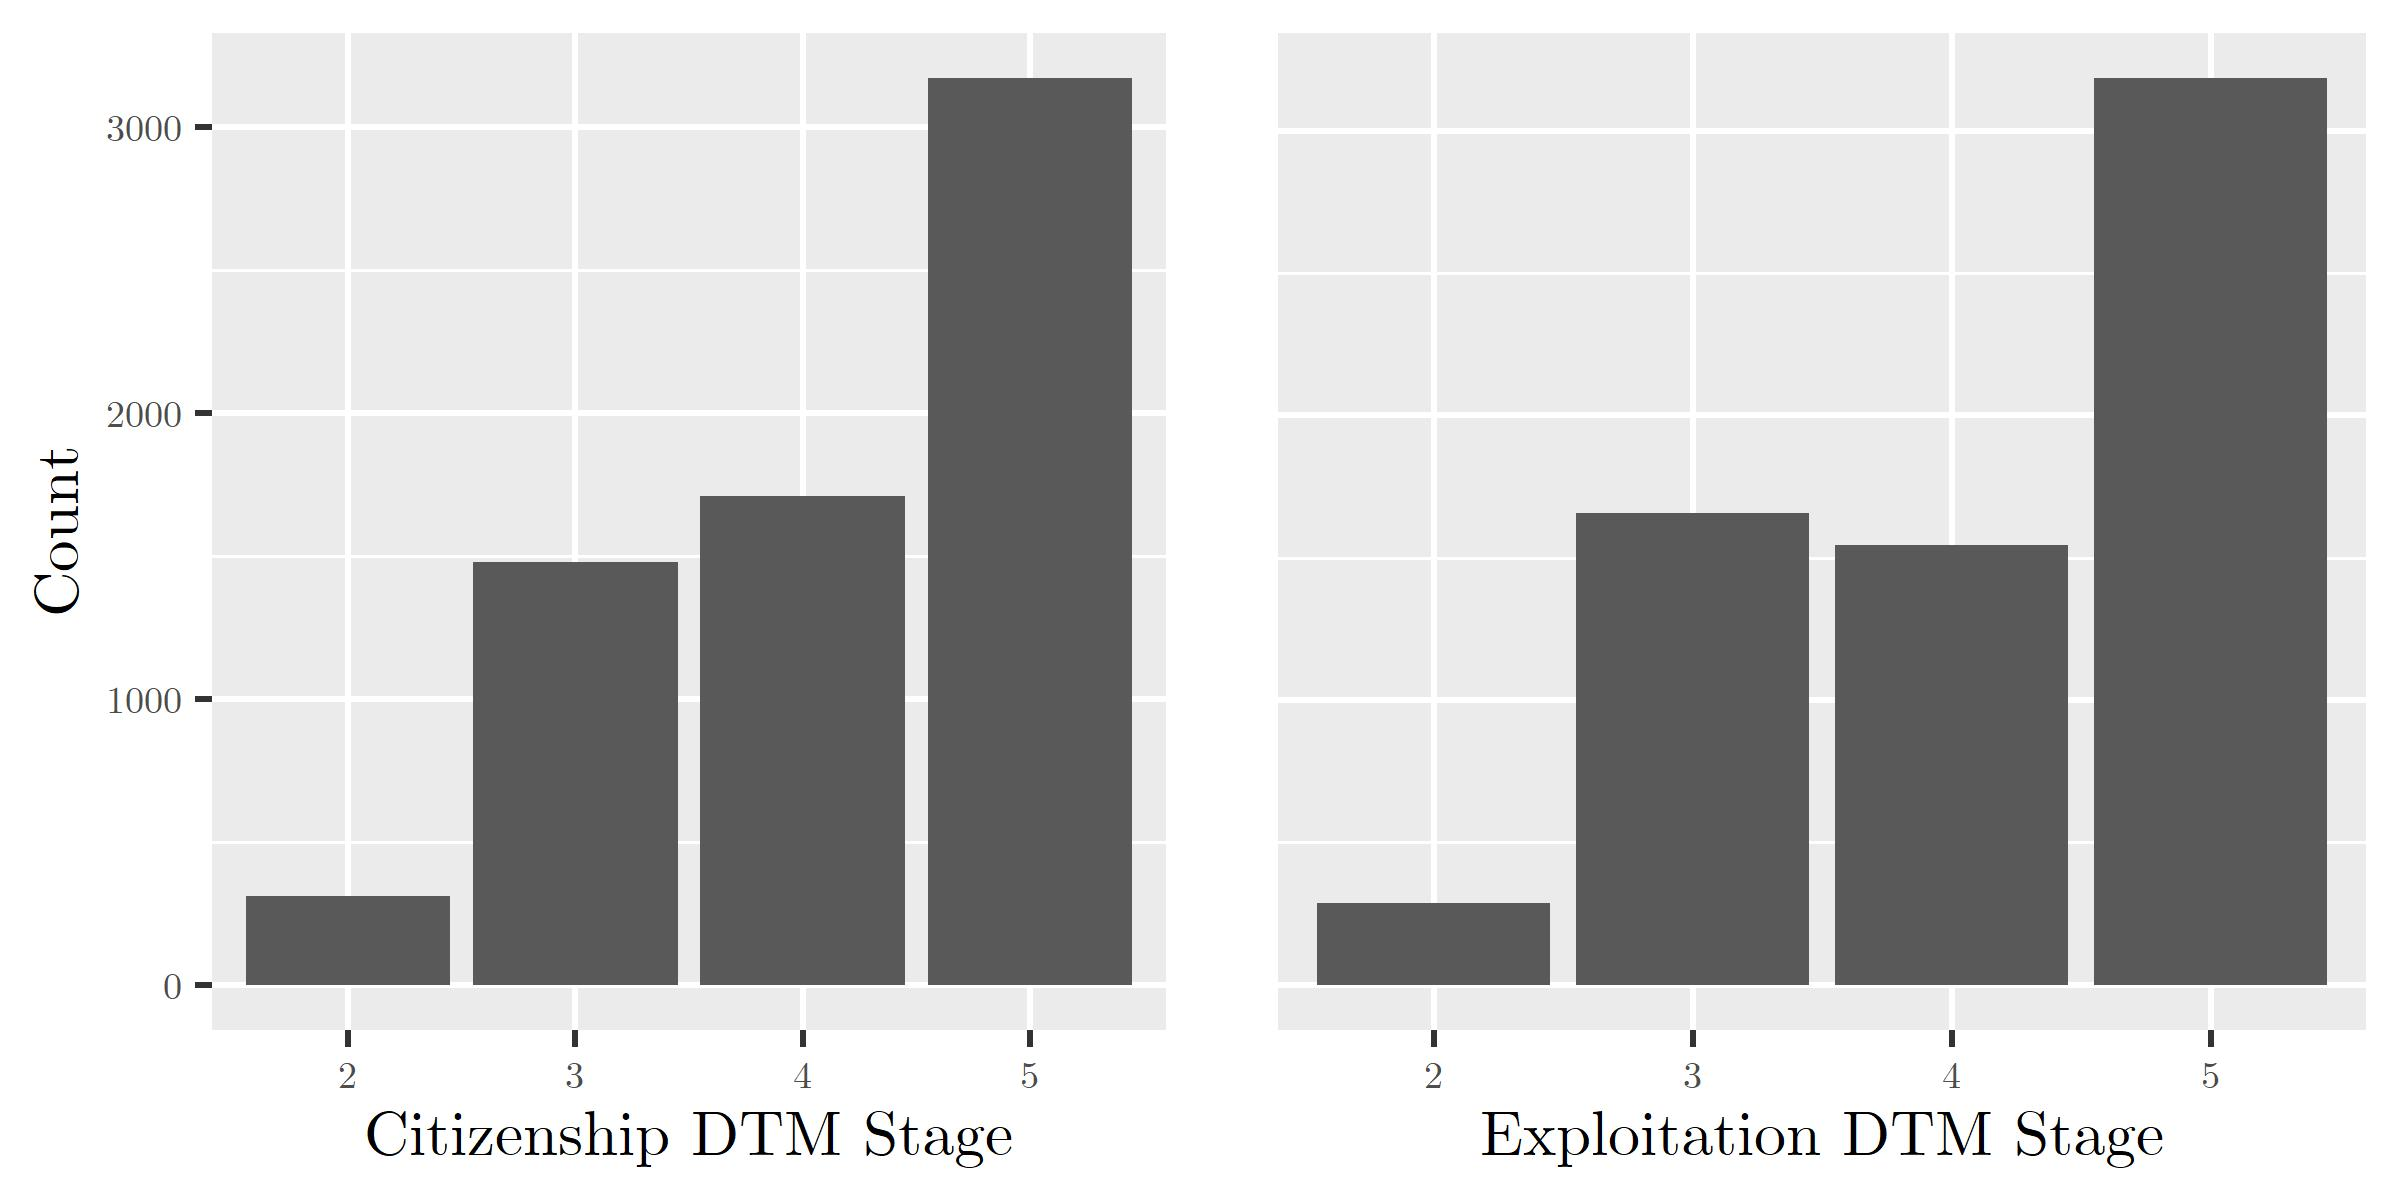
\includegraphics[width=\textwidth]{DTMStagesBarplot}
\end{figure}
\FloatBarrier

In this graphic, one can see that the majority of entries for Citizenship and Exploitation DTM are stage 5, with a decreasing count as the stage decreases. This certainly is interesting, but is something one would expect to see for the DTM stage of exploitation countries. Since these are typically the places in which the victim's case is recorded and added to the CTDC data set, this is not abnormal. One would expect more developed countries to have higher rates of reported cases, as they have access to the resources required to locate the victims. However, this does not explain the trend in Citizenship DTM Stages.
\FloatBarrier
\begin{figure}[H]
	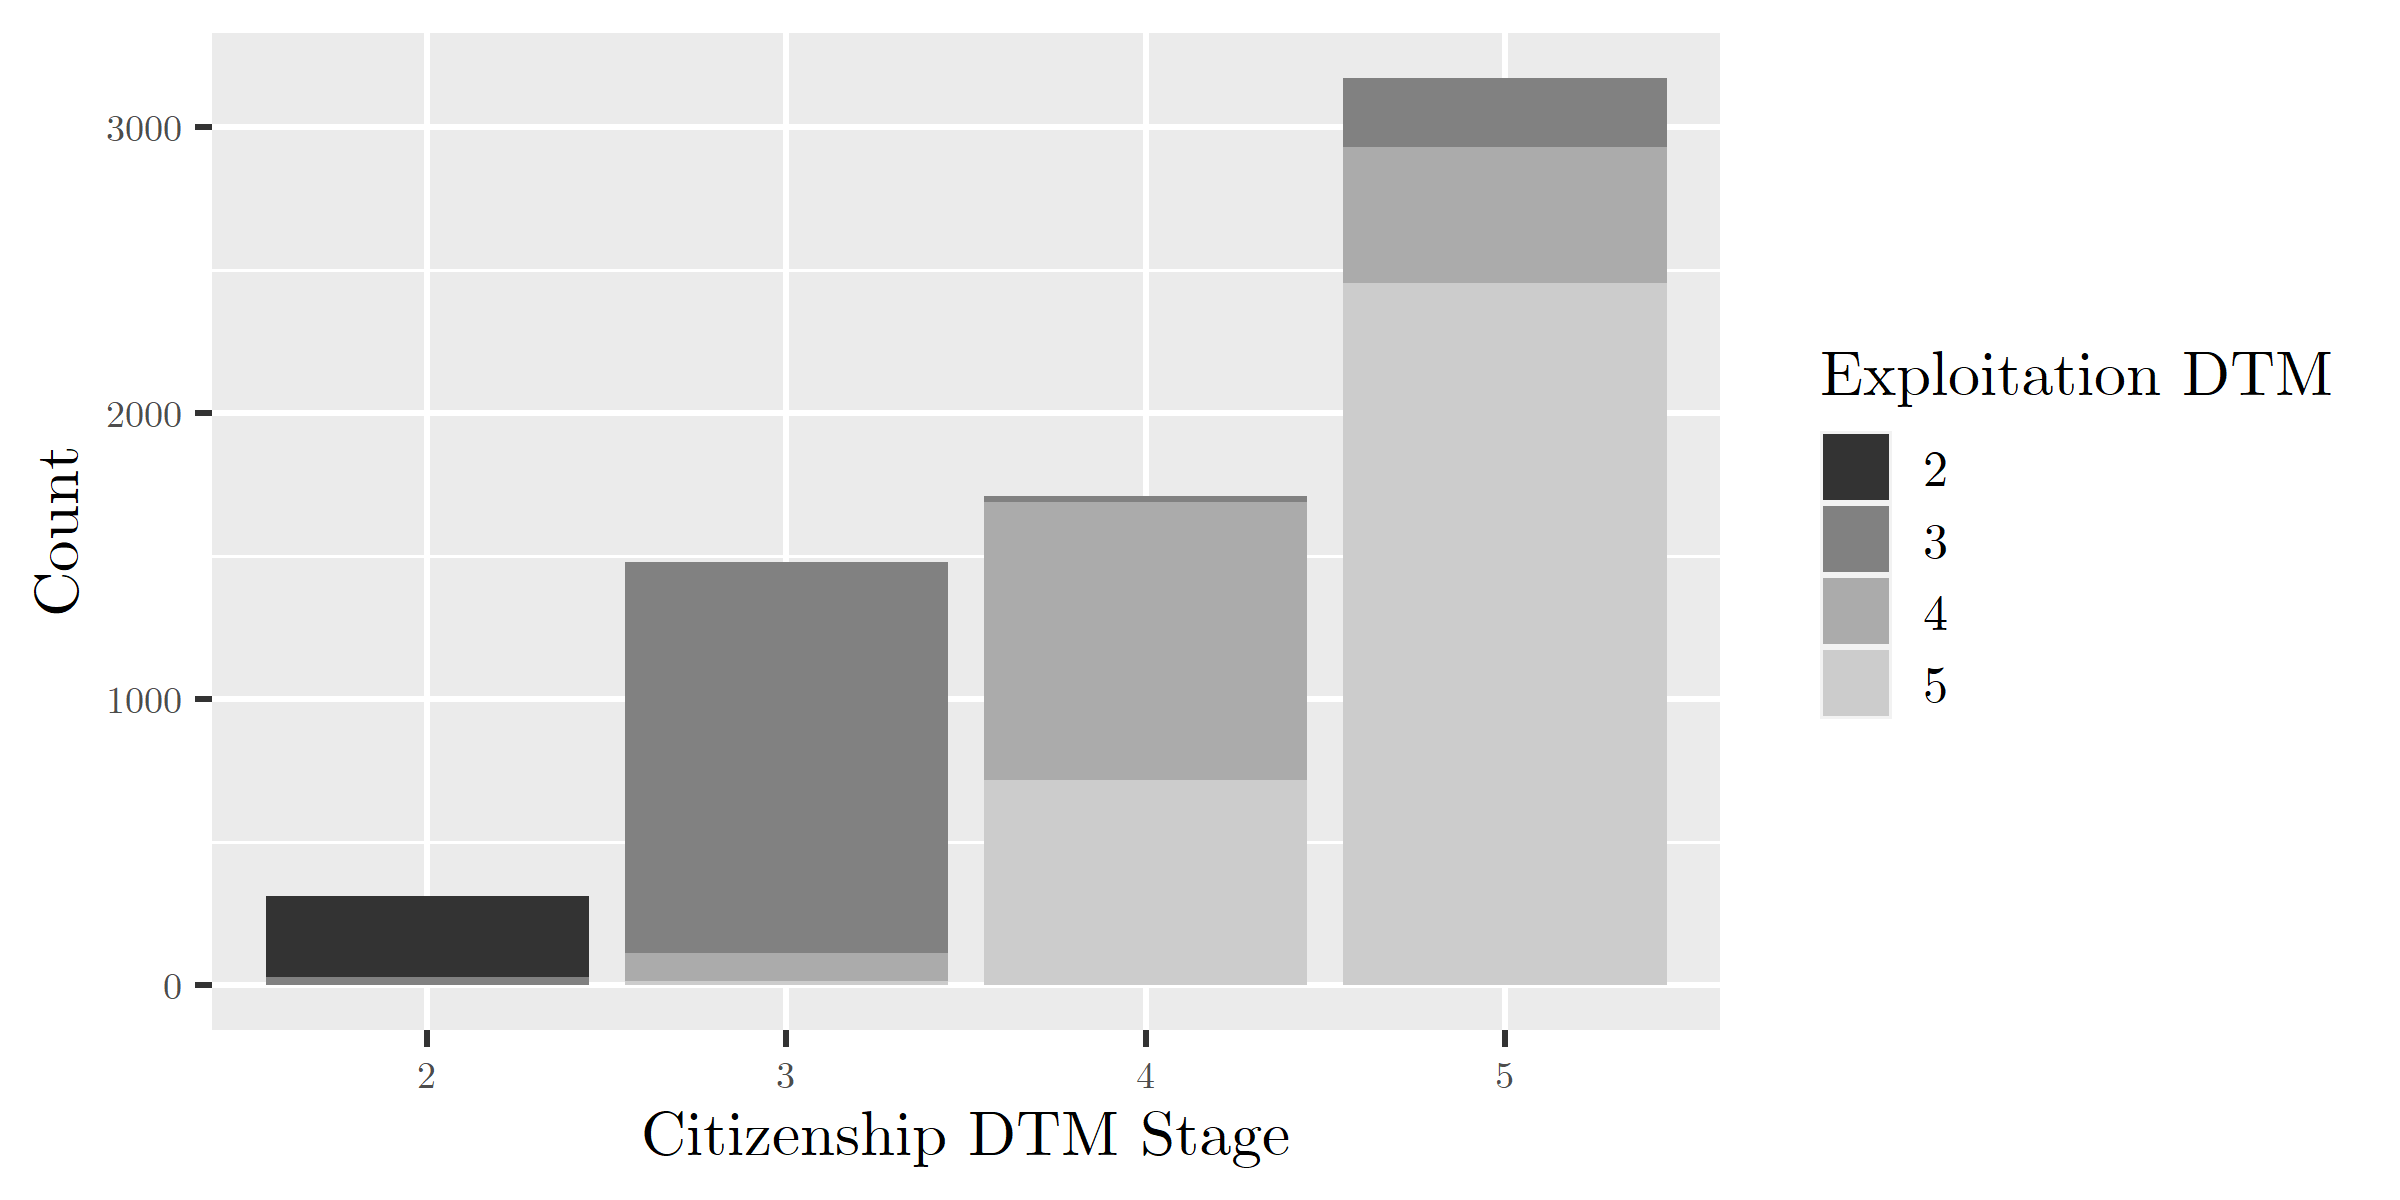
\includegraphics[width = \textwidth]{DTMStage1}
\end{figure}
\FloatBarrier


From this chart, one can see the intersection of the two plots. Each bar has the total count of entries with a certain citizenship DTM stage, and each bar is broken down into the counts of the exploitation DTM stage. For example, one can see that there are roughly 1500 victims with a citizenship DTM stage of 3, and of those, the majority are exploited in a country that is also stage 3.

Of interest in this chart is the fact that for every citizenship DTM stage, the majority of the victims are exploited in a country of the same stage. This pattern can easily be explained by victims typically being exploited in their citizenship country. Further analysis shows that 1,752 of the 6,672 entries (26.3\%) are examples of this. When we remove these entries, the visualization looks like this:

\FloatBarrier
\begin{figure}[H]
	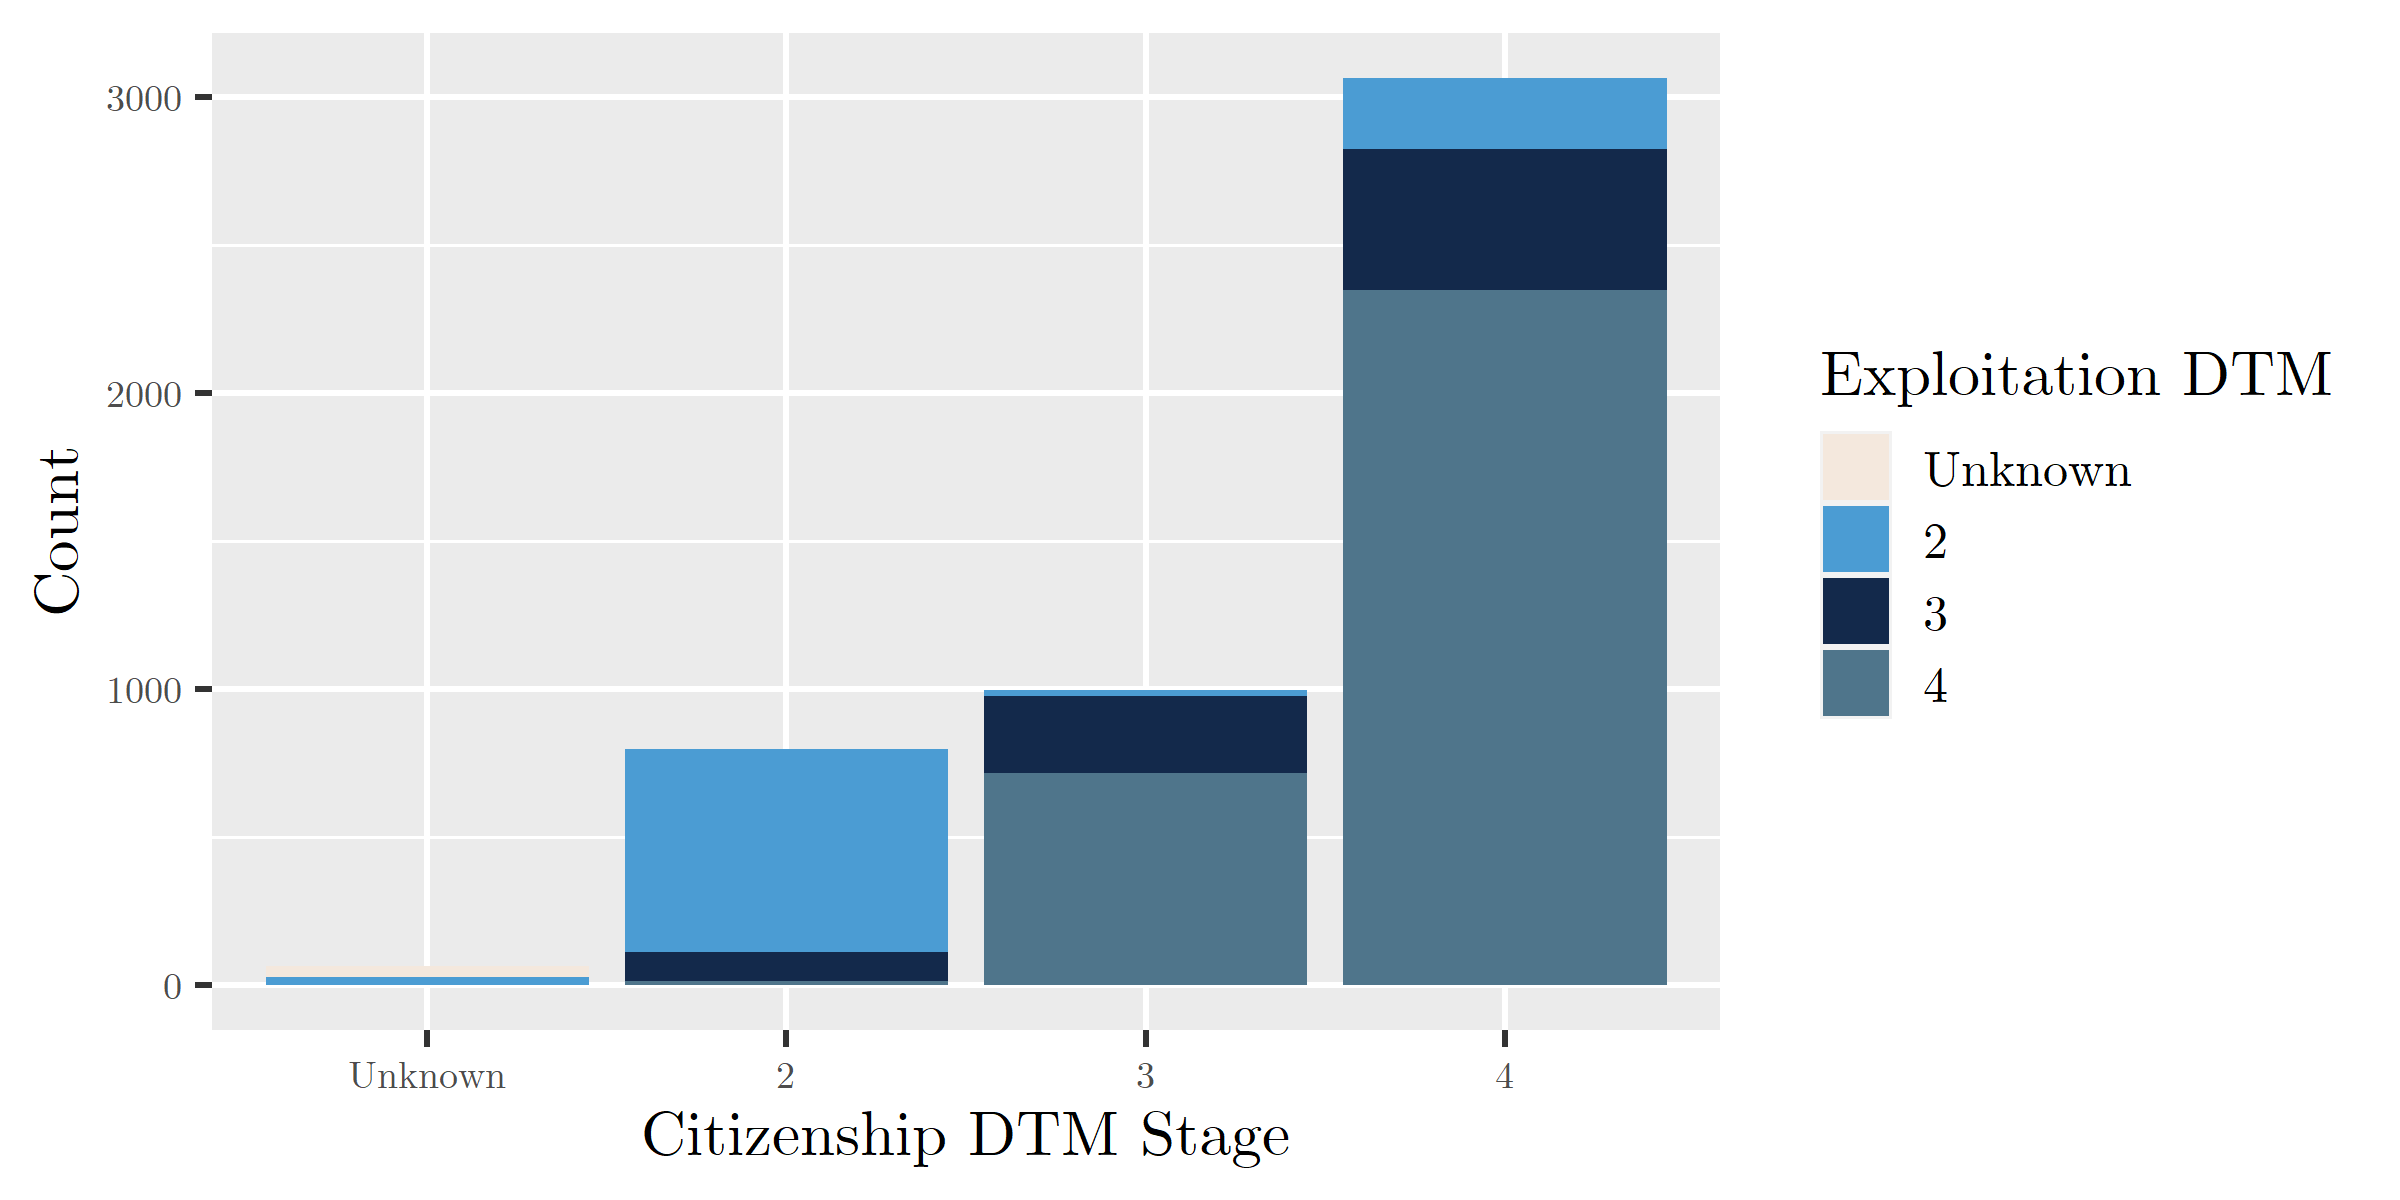
\includegraphics[width = \textwidth]{Different_CountryDTM}
\end{figure}
\FloatBarrier

This image displays a different outcome. Victims from stage 4 countries are more likeley to be exploited in a stage 5 country if they are exploited in a country that is different than their citizenship. However, stages 3 and 5 exhibit the same behavior as before, and citizens from stage 2 countries are split almost evenly between being exploited in stage 2 and 3 countries. Since thevisuals are pretty similar, we can assume that while many victims are exploited in the same country they are a citizen of, there is no evidence to suggest this will have a large impact on the outcome of our model by including these instances. 

Additionally, sine the aim of these models is to inform policy makers, it would make sense to use exploitation DTM stage as the variable of choice, since these correspond to the places in which individuals are actually exploited. However, removing citizenship DTM would remove valuable information for law makers of where the victims in their country are coming from. 
%May not keep the rest of this paragraph%
Some potential ways to counteract this is by assigning a small weight to the citizenship DTM variable, to prevent it from overpowering the rest of the variables in the model. Additionally, adding some random variation to citizenship DTM in our models would lead to the model being more robust. This idea also would be beneficial as it would account for random variation in how DTM stage was determined. Since population pyramids are constantly changing, it is possible there are disagreements on the true DTM classification of a country. For our purposes, each DTM stage in citizenship DTM will either be increased by 1, decreased by 1, or stay the same, with probabilities that will be determined later.



\subsection{More Visualizations}

Since the focus of this research is primarily on the connection between DTM and the typology of human trafficking victims, the following visuals will give more insight into these connections.

\FloatBarrier
\begin{figure}[H]
	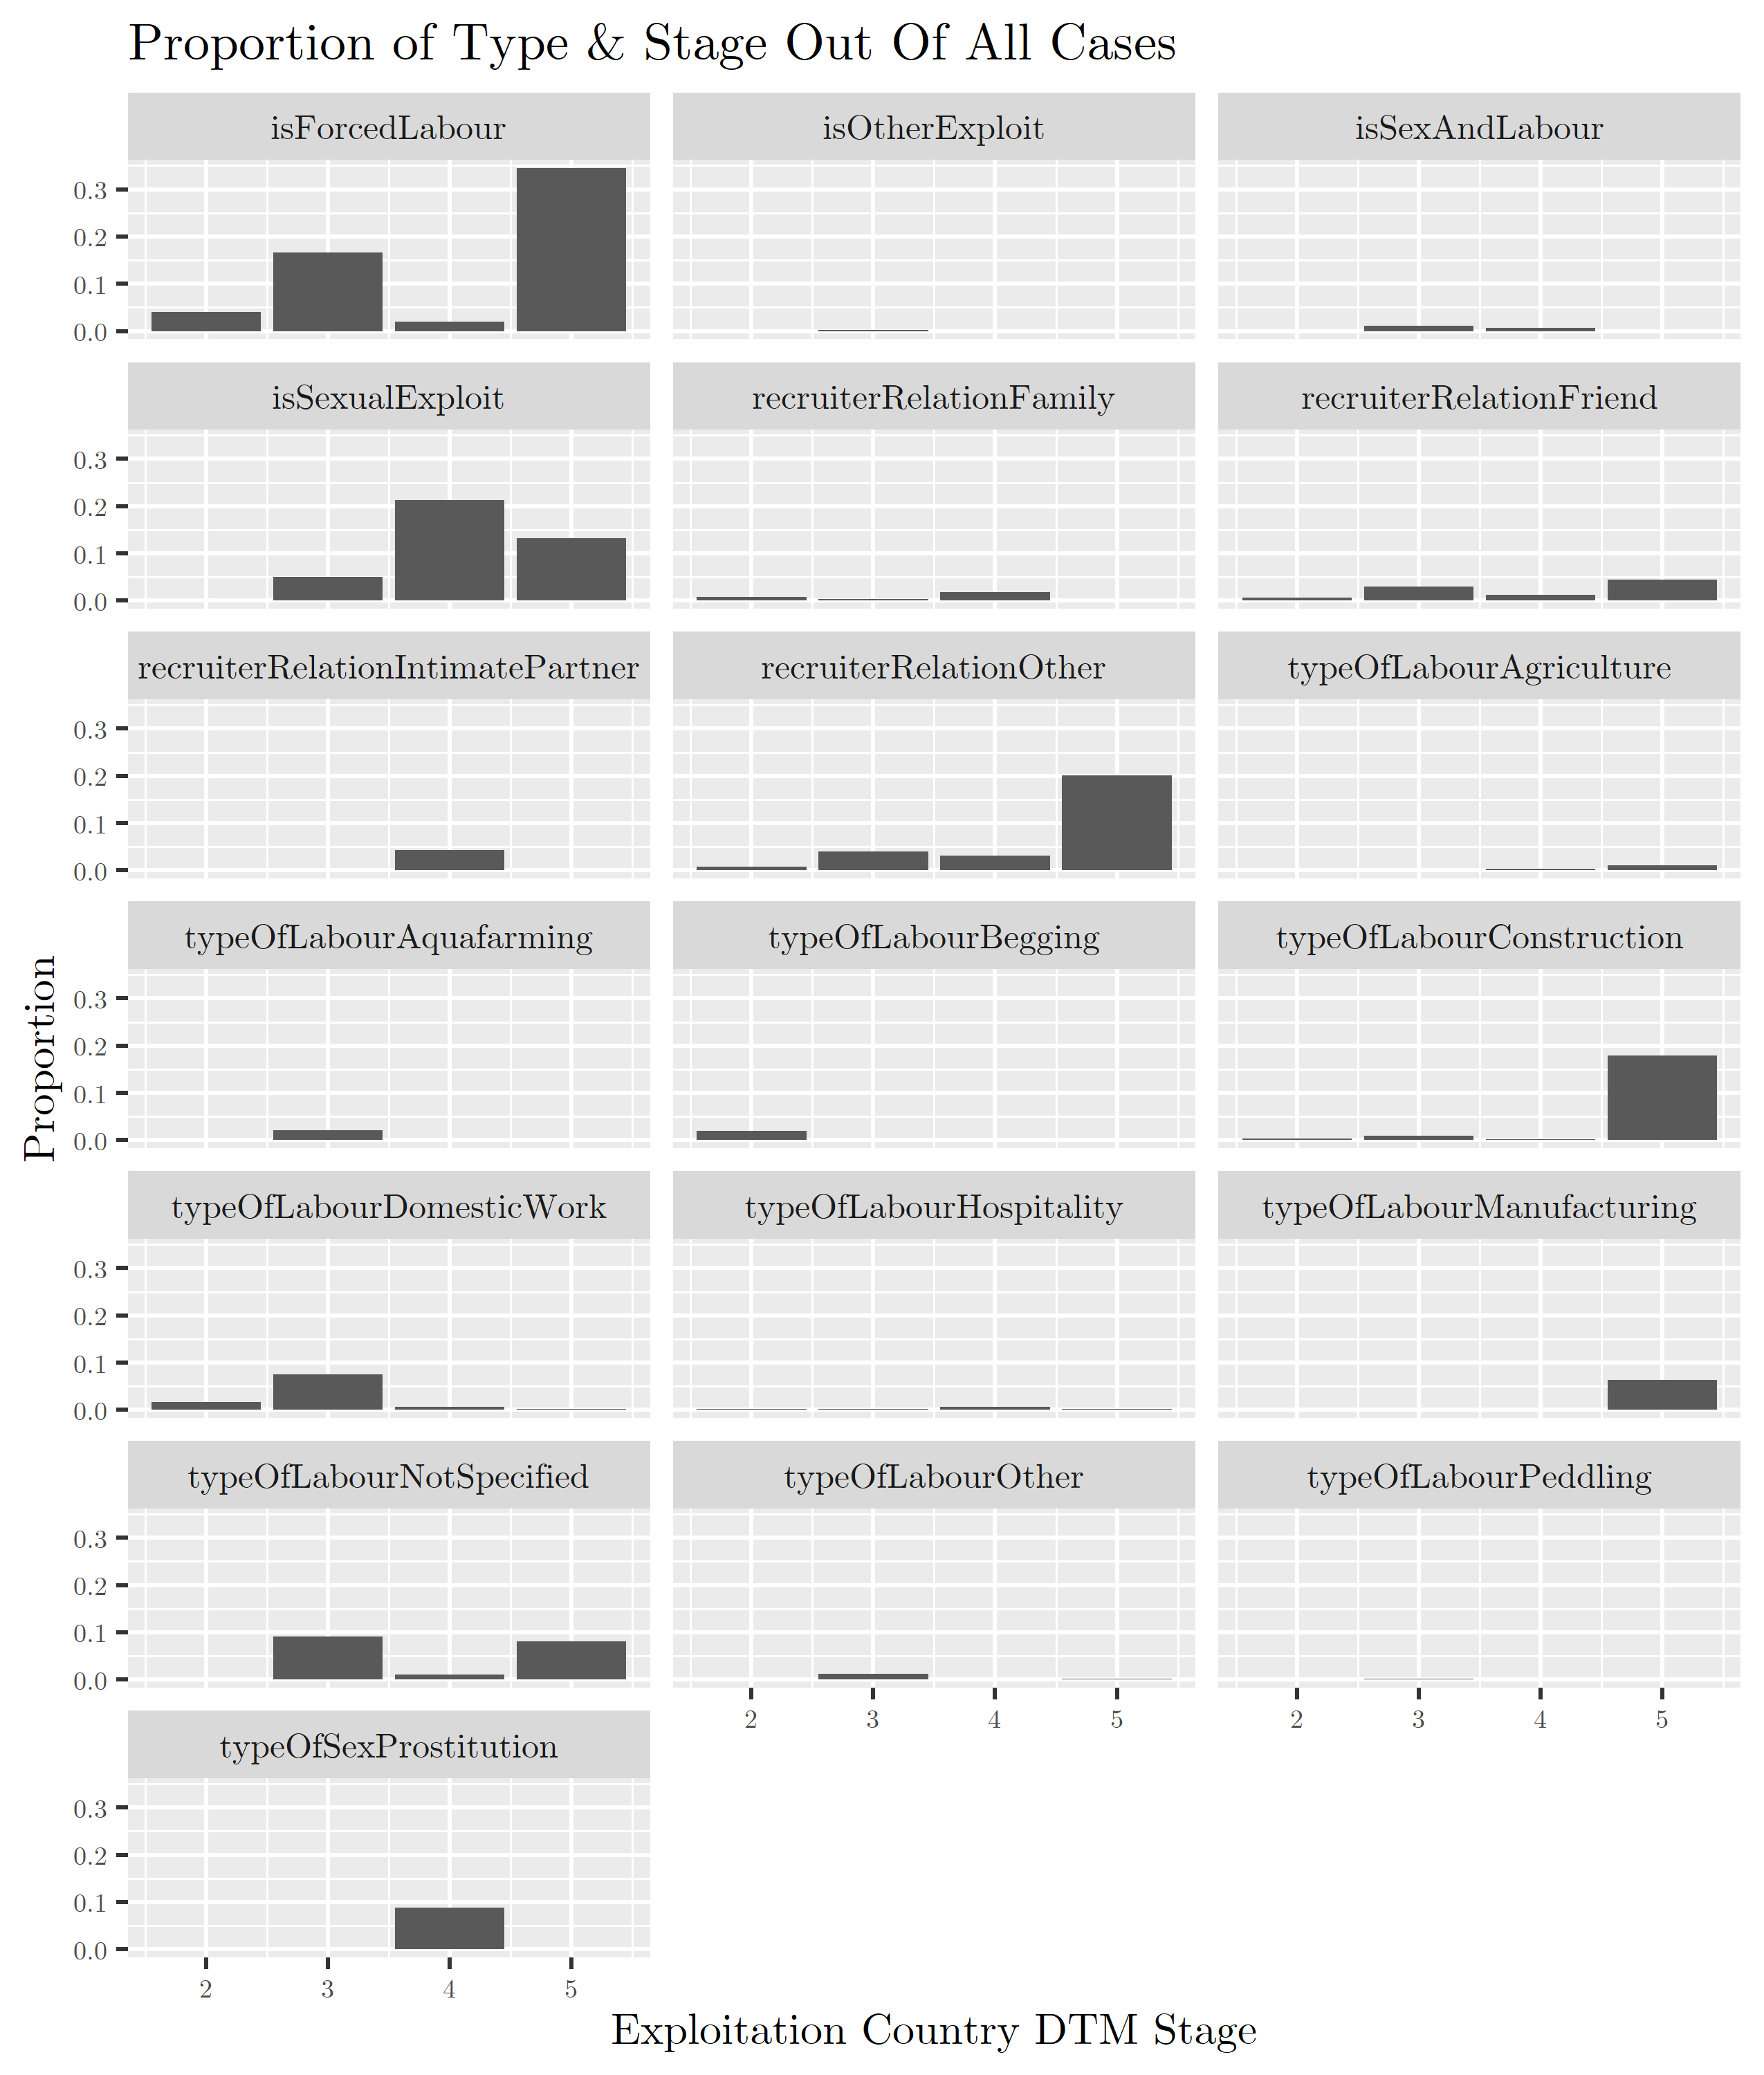
\includegraphics[width = \textwidth]{FacetPlot1}
\end{figure}
\FloatBarrier

In the previous plots, across the bottom axes is the exploitation country DTM stages, and along the vertical axes is the proportion of all human trafficking victims in which the variable is observed. For example, the bottom left plot for "typeOfSexProstitution" tells us that within our data set, approximately 10\% of the cases involve prostitution in a stage 4 country. Additionally, of all cases, it seems as though a minuscule amount of them involve prostitution within countries in stages 2, 3, or 5.

From these plots, we can see some rough trends, like recruiterRelationOther becoming more prominent in more developed countries. The same can be said for typeOfLabourConstruction. Additionally, isSexualExploit seems to have a peak at stage 4 countries, and isForcedLabour peaks in stage 5 countries. One can see how this information can already be of some importance to law makers. Since one can see that sexual exploits peak in stage 4 countries, then if a stage 3 country is about to enter stage 4, it would be useful to know that there will be an increase in sexual exploits within the country.



\printbibliography

\end{document}
